%!TEX program = XeLaTeX 
% 下周: 东主1820, 2:30-4:30
%%%%%%%%%%%%%%%%%%%%%%%%%%%%%%%%%%%%%%%%%%%%%%%%%%%%%%%%%%%%%%%%%%%%%%%%%%%%%%%%%%%%5%%%%%%%%%%%%%%%
%  本文档可在安装了CTEX宏包, CTEX字体下的TEX系统运行,
%  访问http://www.ctex.org, 可以获得最新的宏包与字体安装包
%
%  请使用PDFLATEX对模板编译2次, 可得正确结果, 由于hyperref的设置中不支持DVI-PDF,
%  用LATEX编译时需要替换相应的命令, 详见相应注释.
%
% 文档是在原来李湛、何力同学的模板的基础上修改的, 主要包括以下几个地方:
%
%1.修正了原模板使用hyperref宏包中的设置, 使文档更加美观, 对设置作出了说明, 可以进一步修改
%2.修正了定理的样式, 原定理标题是黑体加粗, 现改为黑体, 原定理正文为倾斜楷体, 现改为楷体, 符合一般论文的格式
%3.对导言区的少部分命令修改, 删去了一些默认的重复的设置
%4.对模板的少部分正文进行充实
%5.对部分原来模板中的注释进行了修改, 删去了不必要的, 加入了一些中文的注释, 方便查阅
%
%  by 张越 Apr.12, 有问题请发送你的问题到:frank_melody@hotmail.com
%%%%%%%%%%%%%%%%%%%%%%%%%%%%%%%%%%%%%%%%%%%%%%%%%%%%%%%%%%%%%%%%%%%%
%%%%%%%%%%%%%%%%%%%%%%%%%%%%%%%%%%%%%%%%%%%%%%%%%%%%%%%%%%%%%%%%%%%%%%
% documentclass can be ctexart, ctexrep, ctexbook, 推荐使用模板中的CTEXREP
% cs4size - 默认的字体大. ∷
% punct - 对中文标点的位置(宽度)进行调整
% twoside - if you want to print on both side of the paper, or else you should omit this

\documentclass[notitlepage,cs4size,punct,oneside]{ctexrep}
% \documentclass[fleqn]{article}
\usepackage{subfig}


% \usepackage{fontspec}
% \setmainfont{Times New Roman}
% \setmainfont{Centaur}
% % \setmainfont{serif}
% \setsansfont{Times New Roman}
% \setmonofont{Times New Roman}


% \usepackage{times}\usepackage[mtbold,mtpluscal,mtplusscr]{mathtime}

% default paper settings, change it according to your word
\usepackage[a4paper,hmargin={2.54cm,2.54cm},vmargin={3.17cm,3.17cm}]{geometry}

\usepackage{amsmath,amssymb,amsthm}
% \usepackage[fleqn]{amsmath}
% 公式编号的计数格式, 在章内计数
\numberwithin{equation}{section}

% set the abstract format, need abstract package

\usepackage[runin]{abstract}

%使用hyperref宏包, 对目录, 公式引用, 文献引用做超链接, 超链接方便电子版的阅读, 但不影响打印
% pdfborder对超链接的边框大小进行设置, 模板中默认边框大小为0
% colorlinks=true, 表示超链接对应的文字采用超链接边框的颜色, =false时保持原字体颜色
% linkcolor=blue, 设置超链接边框的颜色, 可以改为red,green等等.
% CJKbookmarks=true, 生成PDF中文书签,
% 非CTEX套装用户可能发现即便如此设置, 生成的PDF书签也是乱码, 需要用GBK2UNI.EXE解决
\usepackage[pdfborder={0 0 0},colorlinks=true,linkcolor=blue,CJKbookmarks=true]{hyperref}
%若要用LATEX编译, 请用下面的命令替代上述命令:
%\usepackage[dvipdfm,pdfborder={0 0 0},colorlinks=true,linkcolor=blue,CJKbookmarks=true]{hyperref}

\setlength{\absleftindent}{1.5cm} \setlength{\absrightindent}{1.5cm}
\setlength{\abstitleskip}{-\parindent}
\setlength{\absparindent}{0cm}

% Theorem style
\newtheoremstyle{mystyle}{3pt}{3pt}{\kaishu}{0cm}{\heiti}{}{1em}{}
\theoremstyle{mystyle}

\newtheorem{definition}{\hspace{2em}定义}[section]
% 如果没有章, 只有节, 把上面的[chapter]改成[section]
\newtheorem{theorem}[definition]{\hspace{2em}定理}
\newtheorem{axiom}[definition]{\hspace{2em}公理}
\newtheorem{lemma}[definition]{\hspace{2em}引理}
\newtheorem{proposition}[definition]{\hspace{2em}命题}
\newtheorem{corollary}[definition]{\hspace{2em}推论}
\newtheorem{remark}{\hspace{2em}注}[section]
%类似地定义其他“题头”. 这里“注”的编号与定义、定理等是分开的

\def\theequation{\arabic{section}.\arabic{equation}}
\setcounter{equation}{1}
\def\thedefinition{\arabic{section}.\arabic{definition}}

\newcommand{\nq}{\\[5pt]}
\newcommand{\nw}{\\[10pt]}

% title - \zihao{1} for size requirement \heiti for font family requirement

\title{{\zihao{1}\heiti{} 一个随机微分方程组解的统计量}}

\author{卢川\\学号:13300180056\\专业:信息与计算科学}

\date{}

\usepackage{fontspec}
% \setmainfont{Times New Roman}
\setmainfont{Lucida Bright} 
% \setmainfont{Segoe Script}
\setsansfont{Lucida Bright} 
\setmonofont{Lucida Bright} 
% \setsansfont{Segoe Script}
% \setmonofont{Segoe UI }

%%%%%%%%%%%%%%%%%%%导言区设置完毕
%%%%%%%%%%%%%%%%%%%%%%%%%%%%%%%%%%%%%%%%%%%%%%%%%%%%%%%%%%%%%%%%%%%%%
\begin{document}

%Styles for chapters/section
%若要将章标题左对齐, 用下面这个语句替换相应的设置
%\CTEXsetup[nameformat={\raggedright\zihao{3}\bfseries},%
\CTEXsetup[nameformat={\zihao{3}\heiti},%
           titleformat={\zihao{3}},%
           beforeskip={0.8cm},afterskip={1.2cm}]{chapter}
\CTEXsetup[nameformat={\zihao{4}\bfseries},%
           titleformat={\zihao{4}},%
           name={第~,~节},number={\arabic{section}},%
           beforeskip={0.4cm},afterskip={0.4cm}]{section}
\CTEXsetup[format={\zihao{-4}\bfseries},%
           titleformat={\zihao{-4}},%
           number={\arabic{section}.\arabic{subsection}},%
           beforeskip={0.4cm},afterskip={0.4cm}]{subsection}
\CTEXsetup[format={\zihao{-4}\bfseries},%
           titleformat={\zihao{-4}},%
           number={\arabic{section}.\arabic{subsection}.\arabic{subsubsection}},%
           beforeskip={0.4cm},afterskip={0.4cm}]{subsubsection}
\CTEXoptions[abstractname={摘要:}]
\CTEXoptions[bibname={\heiti 参考文献}]

\renewcommand{\thepage}{\roman{page}}
\setcounter{page}{1}
\tableofcontents\clearpage

\maketitle\renewcommand{\thepage}{\arabic{page}}
\thispagestyle{empty}\setcounter{page}{1}
%%%  论文的页码从正文开始计数, 摘要页不显示页码
% 撰写论文的摘要


\newcommand{\Var}{\text{Var}}
\newcommand{\E}{\text{E}}
\newcommand{\Cov}{\text{Cov}}

\begin{abstract}
本文研究了一个用于改进Kalman滤波结果的重要随机微分方程组的解, 利用It\^o积分和特征函数补全了解的一阶和二阶统计量的计算过程, 并对理论结果进行了数值检验. \\

\noindent{\heiti 关键字:} 随机微分方程组; 统计量; It\^o积分
\end{abstract}

\section{导言}
\subsection{问题简介}
在对Kalman滤波的结果进行改进时, 研究者提出了如下的一个随机微分方程组来模拟现实中常见的随机信号\cite{gershgorin2010test}:
\begin{equation} \label{E0}
\left\{
\begin{split}
& \frac{du(t)}{dt} = (-\gamma(t)+i\omega)u(t)+b(t)+f(t)+\sigma W(t), \\[5pt]
% \end{equation}
% \begin{equation}
& \frac{db(t)}{dt} = (-\gamma_b+i\omega_b)(b(t)-\hat{b})+\sigma_b W_b(t), \\[5pt]
% \end{equation}
% \begin{equation}
& \frac{d\gamma(t)}{dt} = -d_\gamma(\gamma(t)-\hat{\gamma})+\sigma_\gamma W_\gamma(t)
\end{split}
\right.
\end{equation}

其中$\omega$为$u(t)$的振荡频率, $f(t)$为外部驱动力, $\sigma$表示白噪声$W(t)$的强度. 此外, 参数$\gamma_b$和$d_\gamma$表示振荡阻尼, $\sigma_b$和$\sigma_\gamma$分别表示加性和乘性修正((\ref{E0})中第2, 3式)中白噪声的强度. $\hat{b}$和$\hat{\gamma}$分别表示$b(t)$和$\gamma(t)$的固定平均偏差修正, $\omega_b$表示加性噪声的频率. 白噪声$W_\gamma(t)$是实值函数, 而$W(t)$及$W_b(t)$均为复值, 且其实部和虚部均为独立的白噪声. 

一般认为方程组(\ref{E0})有初值
\begin{equation} \label{init_values}
\left\{
\begin{split}
& u(t_0) = u_0, \\[5pt]
& b(t_0) = b_0, \\[5pt]
& \gamma(t_0) = \gamma_0,
\end{split}
\right.
\end{equation}
且$u_0$, $b_0$, $\gamma_0$均为独立的高斯随机变量, 其统计量
$\E[u_0]$, ~$\E[\gamma_0]$, ~$\E[b_0]$, ~$\Var(u_0)$, ~$\Var(\gamma_0)$, ~$\Var(b_0)$, ~$\Cov(u_0, u_0^*)$, ~$\Cov(u_0, \gamma_0)$, ~$\Cov(u_0, b_0)$, ~$\Cov(u_0, b_0^*)$均假设为已知.

(\ref{E0})的第二和第三项均为线性方程, 由求解线性常微分方程组的相关知识\cite{fulinjin1984ordinary}可知其通解有以下的形式:
\begin{equation} \label{Sb}
\begin{split}
&b(t) = \hat{b}+(b_0-\hat{b})e^{\lambda_b(t-t_0)}+\sigma_b\int_{t_0}^t e^{\lambda_b(t-s)}dW_b(s), \\[5pt]
&\gamma(t) = \hat{\gamma}+(\gamma_0-\hat{\gamma})e^{-d_{\gamma}(t-t_0)}+\sigma_{\gamma}\int_{t_0}^t e^{-d_{\gamma}(t-s)}dW_{\gamma}(s).
\end{split}
\end{equation}

其中$\lambda_b = -\gamma_b+i\omega_b$.
如果我们记
\begin{equation} \label{def J(s, t)}
\begin{split}
&\hat{\lambda} = -\hat{\gamma}+i\omega, \\[5pt]
&J(s, t) = \int_s^t (\gamma(s')-\hat{\gamma})ds'
\end{split}
\end{equation}

则(\ref{E0})的通解可以表示为
\begin{equation} \label{Su}
\begin{split}
u(t) &= e^{-J(t_0, t)+\hat{\lambda}(t-t_0)}u_0 + \int_{t_0}^t (b(s)+f(s))e^{-J(s, t)+\hat{\lambda}(s-t_0)}ds \\[5pt]
& + \sigma\int_{t_0}^{t}e^{-J(s, t)+\hat{\lambda}(s-t_0)}dW(s).
\end{split}
\end{equation}
本文在第三和第四节中将对方程(\ref{E0})的各个变量$u, ~b, ~\gamma$, 分别计算其一阶和二阶统计量, 以及各个变量间的相关性.

\section{一些前置引理}
\subsection{布朗运动的性质}
在应用中, 往往将布朗运动置于随机微分方程中, 以模拟白噪声的性质\cite{hida1980brownian}. 
为了简化计算过程, 我们在这里引入布朗运动的一些基本性质\cite{oksendal2003stochastic}\cite{nelson1967dynamical}.
\begin{theorem} \label{brownian1}
布朗运动$B_t$是一个Gaussian过程. 即对于所有的$0 \leqslant t_1 \leqslant\cdots\leqslant t_k$, 随机向量$Z = (B_{t_1}, B_{t_2}\cdots ,B_{t_k})\in \mathbb{R}^{nk}$ 服从多维正态分布. 如果设$B_{t_i}$的初值均为$x$, 则此随机向量的期望为 
$$M = \E[Z] = (x, x, \cdots, x) \in \mathbb{R}^{nk},$$
协方差矩阵为
$$C = \left(\begin{matrix}
			t_1I_n & t_1I_n & \cdots & t_1I_n \\
			t_1I_n & t_2I_n & \cdots & t_2I_n \\
			\vdots & \vdots & \ddots & \vdots \\
			t_1I_n & t_2I_n & \cdots & t_kI_n 
			\end{matrix}
			\right).$$
\end{theorem}

此定理的证明利用了正态分布特征函数的性质, 具体过程可见\cite{oksendal2003stochastic}的附录A. 以下是定理(\ref{brownian1})的直接而显然的推论:
\begin{theorem}
假设布朗运动$B_t$满足定理(\ref{brownian1})中的条件, 那么当$t\geqslant 0$时,
$$\E[B_t] = x, ~\E\left[(B_t - x)^2\right] = nt, ~\E[(B_t - x)(B_s - x)] = n\min(s, t).$$ 
而且如果$t \geqslant s$, 有$\E\left[(B_t - B_s)^2\right] = n(t-s)$.
\end{theorem}

以下的定理也是布朗运动的一个重要性质, 其证明见\cite{oksendal2003stochastic}的(2.2.12)式.
\begin{theorem}
$B_t$有独立的增量, 即对满足$\forall 0 \leqslant t_1 < t_2 \cdots < t_k$的$(t_1, t_2, \cdots t_k)$,
$$B_{t_1}, ~B_{t_2}-B_{t_1}, ~\cdots, ~B_{t_k}-B_{t_{k-1}}$$相互独立.
\end{theorem}

\subsection{It\^{o}积分及其性质}
在求解类似(\ref{E0})的随机微分方程时, 需要针对布朗运动做积分, 为此我们需要引入以下的It\^{o}积分\cite{oksendal2003stochastic}\cite{lawler2006introduction}:
\begin{definition}(It\^{o}积分)	设$f\in\mathcal{V}(S, T)$. 则$f$的It\^{o}积分定义为
$$\int_S^T f(t, \omega)dB_t(\omega) = \lim_{n\to\infty}\int_S^T\phi_n(t, \omega)dB_t(\omega),$$
其中${\phi_n}$为基本函数序列, 且满足当$n \to \infty$时
$$\E\left[\int_S^T (f(t, \omega)-\phi_n(t, \omega))^2dt\right] \to 0.$$
\end{definition}

由上述定义即可得到It\^{o}积分的一个重要性质:
\begin{theorem} \label{Ito isometric} (It\^{o}等距) 对于$\forall f\in\mathcal{V}(S, T)$有
$$\E\left[\left(\int_S^T f(t, \omega)dB_t\right)^2\right] = \E\left[\int_S^T f^2(t, \omega)dt\right].$$
\end{theorem}

这里$\mathcal{V}(S, T)$见\cite{oksendal2003stochastic}中的定义3.1.2至3.1.4. \\
利用上述方法, 即利用基本函数序列来逼近$\mathcal{V}(S, T)$中的函数, 我们能够得到It\^{o}积分的线性性质:
\begin{theorem} \label{Itoint_property}
设$f, g \in \mathcal{V}(0, T)$, $0 \leqslant S < U < T$. 那么
\begin{flalign*}
& (1)\quad \int_S^T fdB_t = \int_S^U fdB_t + \int_U^T fdB_t, ~\text{a.e.}\\[5pt]
& (2)\quad \int_S^T (cf+g)dB_t = c\int_S^T fdB_t + \int_S^T gdB_t, ~\text{a.e.}\\[5pt]
& (3)\quad \E\left[\int_S^T fdB_t\right] = 0.
\end{flalign*}
\end{theorem}

我们还需要引入以下的一维It\^{o}公式\cite{jiangangying2016stochastic}来计算一维情形的It\^o积分.
\begin{theorem}(It\^{o}公式) \label{Ito formula} 设$X_t$为一个如下的It\^{o}过程:
$$dX_t = udt+vdB_t,$$
$g(t, x) \in C^2\left([0, \infty) \times \mathbb{R}\right)$, 则$Y_t = g(t, X_t)$也是一个It\^{o}过程, 且满足:
$$dY_t = \frac{\partial g}{\partial t}(t, X_t)dt + \frac{\partial g}{\partial x}(t, X_t)dX_t + \frac{1}{2}\frac{\partial^2 g}{\partial x^2}(t, X_t)\cdot(dX_t)^2,$$
其中
$$dt\cdot dt = dt\cdot dB_t = dB_t\cdot dt = 0, ~dB_t\cdot dB_t = dt.$$
\end{theorem}

以下是上述It\^{o}公式的积分形式.
\begin{theorem} \label{Itoint}(分部积分) 设$f(s, \omega)$对几乎所有的$\omega$关于$s\in [0, t]$是连续的, 且为有界变差函数, 则有
$$\int_0^t f(s)dB_s = f(t)B_t - \int_0^t B_s df_s.$$
\end{theorem}
上述几个定理的证明请见\cite{oksendal2003stochastic}, 21-24页及36-39页. \\

\subsection{高斯分布, 复高斯分布与特征函数}
在问题的假设中, 各个噪声信号均服从高斯分布, 为此我们需要知道多元高斯分布的概率密度\cite{shuyuanhe2006probability}.
\begin{proposition} \label{multiVariable gaussian pdf}
如果随机向量$\textbf{X}$服从多元正态分布
$$\textbf{X} \sim \mathcal{N}(\mu, \Sigma),$$
那么$\textbf{X}$的概率密度为
$$f_\textbf{X}(X_1, \cdots, X_k) = \frac{\exp\left(-\frac{1}{2}(\textbf{X}-\mu)^\top\right)\Sigma^{-1}(\textbf{X}-\mu)}{\sqrt{(2\pi)^k|\Sigma|}}$$
\end{proposition}
对于一个复值的Gauss变量$X = a+bi$, 其中$a$与$b$均服从Gauss分布, 那么其期望和方差为
\[
\begin{split}
&\E[X] = \E[a] + i\E[b], \\[5pt]
&\Var(X) = \E[(X-\E[X])(X-\E[X])^*]
\end{split}
\]

除此之外, 我们还需要引入随机变量的特征函数这个工具, 用于计算较为复杂的随机变量的统计量.
\begin{definition}(特征函数) 如果$X$是实值随机变量, $\E[\sin(tX)], ~\E[\cos(tX)]$均存在, 那么称
$$\phi(t) = \E\left[e^{itX}\right] = \E[\cos(tX)] + i\E[\sin(tX)], ~t\in \mathbb{R}$$
为$X$的特征函数, 其中$i$为虚数单位.
\end{definition}
对于随机向量, 其特征函数定义为
\begin{definition} 设$\textbf{X} = (X_1, X_2, \cdots, X_n)$为随机向量, 则$\textbf{X}$的特征函数为
$$\phi(t) = \E\left[\exp(i\textbf{t}\textbf{X}^\top)\right], ~\textbf{t} = (t_1, t_2, \cdots, t_n)\in \mathbb{R}^n.$$
\end{definition}
以下为高斯分布的特征函数.
\begin{proposition} \label{Characteristic function of Gaussian Distribution}
Gauss分布$N(\mu, \sigma^2)$的特征函数为
$$\phi(t) = \exp(i\mu t - \frac{1}{2}\sigma^2t^2)$$
\end{proposition}
此命题的证明见\cite{shuyuanhe2006probability}第五章例2.4.
一个更一般的定义如下\cite{jiangangying2013probability}:
\begin{definition} \label{characteristic function definition 2} 设$\xi$为d-维随机变量, $F$为$\xi$的分布函数. 那么
$$\hat{F}(x) = \int_{\mathbb{R}^d} e^{ix\cdot y}dF(y), ~x\in \mathbb{R}^d$$
(其中$(\cdot)$为$\mathbb{R}^d$空间中的内积) 称为分布函数$F$的特征函数.
\end{definition}
由此定义即可看出, 特征函数即为概率密度函数的Fourier变换:
\begin{equation} \label{characteristic function definition 3}
\hat{F}(x) = \int_{\mathbb{R}^d}e^{ix\cdot y}f(y)dy.
\end{equation}

以下是Fourier变换的一个基本性质, 在求$u(t)$的统计量时将会用到\cite{boggess2015first}.
\begin{proposition}(Fourier变换的微分关系) \label{Fourier transform property 1}
如果
$$\lim_{|x|\to\infty} f(x) = 0,$$
且$f'(x)$的Fourier变换存在, 那么
$$\mathcal{F}[f'(x)] = i\omega\mathcal{F}[f(x)].$$
更一般的, 若
$f(\infty) = f'(\infty) = \cdots = f^{(k-1)}(\infty) = 0,$ 且$\mathcal{F}[f^{(k)}(x)]$存在, 则
$$\mathcal{F}[f^{(k)}(x)] = (i\omega)^k \mathcal{F}[f].$$
\end{proposition}

\section{$b(t)$与$\gamma(t)$的统计量}
\subsection{均值}
当t固定时, 由(\ref{Sb})式可知$b(t)$的通解第一项为常数, 第二项中只有$b_0$是一个随机变量. 那么由(\ref{init_values})可知, $b(t)$通解第二项的期望为$(\E[b_0]-\hat{b})e^{\lambda_b(t-t_0)}$. 而由于
$$f = f(s) = e^{\lambda_b(t-s)}\in\mathcal{V}(S, T),$$
故由(\ref{Itoint_property})的(3)式可知,
$$\E\left[\sigma_b\int_{t_0}^{t} e^{\lambda_b(t-s)dW_b(s)}\right] = 0.$$
从而
\begin{equation} \label{b_stat_1}
\E(b(t)) = \hat{b} + (\E[b_0] - \hat{b})e^{\lambda_b(t-t_0)}.
\end{equation}

对于$\gamma$亦有相同的结论
\begin{equation} \label{gamma_stat_1}
\E(\gamma(t)) = \hat{\gamma} + (\E[\gamma_0] - \hat{\gamma})e^{-d_{\gamma}(t-t_0)}.
\end{equation}

\subsection{方差}
当t固定时, $b(t)$为一个复值随机变量, 由\cite{shuyuanhe2006probability}的第四章相关知识,
 % 考虑到$(b_0-\hat{b})e^{\lambda_b(t-t_0)}$与$\sigma_b\int_{t_0}^t e^{\lambda_b(t-s)}dW_b(s)$相互独立(由(\ref{init_values})可知),
\begin{equation} \label{b_stat_2_process}
\begin{split}
\text{Var}&(b(t)) = \E\left[(b(t)-\E[b(t)])(b(t)-\E[b(t)])^*\right] \\[10pt]
&= \E\left[\left((b_0-\E[b_0])e^{\lambda_b(t-t_0)}+\sigma_b\int_{t_0}^t e^{\lambda_b(t-s)}dW_b(s)\right)\times\right. \\[5pt]
&\quad\quad\left.\left((b_0-\E[b_0])e^{\lambda_b(t-t_0)}+\sigma_b\int_{t_0}^t dW_b(s) \right)^*\right] \\[5pt] 
&= e^{-2\gamma_b(t-t_0)}\Var(b_0) + \E\left[\sigma_b^2\int_{t_0}^t e^{\lambda_b(t-s)}dW_b(s)\left(\int_{t_0}^t e^{\lambda_b(t-s)}dW_b(s)\right)^*\right] \\[5pt]
&= e^{-2\gamma_b(t-t_0)}\Var(b_0) + \sigma_b^2\E\left[\int_{t_0}^t e^{-2\gamma_b(t-s)}ds\right]
\end{split}
\end{equation}

上面的最后一式右边利用了It\^{o}等距(\ref{Ito isometric}).
计算右边即可得到
\begin{equation} \label{b_stat_2} 
\Var(b(t)) = e^{-2\gamma_b(t-t_0)}\Var(b_0) + \frac{\sigma_b^2}{2\gamma_b}(1-e^{-2\gamma_b(t-t_0)}).
\end{equation}

同样的, 我们也有
\begin{equation} \label{gamma_stat_2}
\Var(\gamma(t)) = e^{-2d_\gamma(t-t_0)}\Var(\gamma_0) + \frac{\sigma_\gamma^2}{2d_\gamma}(1-e^{-2d_\gamma(t-t_0)}).
\end{equation}

\subsection{协方差}
考虑到$b(t)$为复值函数, 由协方差的定义\cite{shuyuanhe2006probability}即可知
\[
\begin{split}
\Cov&(b(t), b(t)^*) = \E\left[(b(t) - \E[b(t)])(b(t)^* - \E[b(t)^*])\right] \\[10pt]
&= \E\left[(b_0 - \E[b_0]e^{\lambda_b (t-t_0)}+\sigma_b\int_{t_0}^{t} e^{\lambda_b (t-s)}dW_b(s))\right. \times \\[5pt]
&\quad \left.((b_0^* - \E[b_0^*])e^{\lambda_b(t-t_0)}+\sigma_b\int_{t_0}^t e^{\lambda_b (t-s)}dW_b(s))\right] \quad\quad\quad\quad\quad\quad\quad\cdots(\ref{b_stat_1}) \\[5pt]
&= \E\left[(b_0 - \E[b_0])(b_0^* - \E[b_0^*])e^{2\lambda_b (t-t_0)}\right] + \sigma_b\E\left[(b_0 - \E[b_0])\int_{t_0}^{t}e^{\lambda_b(t-s)}dW_b(s)\right]\\[10pt]
&\quad+ \sigma_b\E\left[(b_0^*-\E[b_0^*])e^{\lambda_b(t-t_0)}\int_{t_0}^{t}e^{\lambda_b(t-s)}dW_b(s)\right] + \sigma_b^2\E\left[(\int_{t_0}^{t}e^{\lambda_b(t-s)}dW_b(s))^2\right]
\end{split}
\]

在上式的第二项中, 由于$b_0$与$\int_{t_0}^{t} e^{\lambda_b (t-s)}dW_b(s)$相互独立, 故由It\^{o}积分的性质(\ref{Itoint_property})可知
\[
\sigma_b\E\left[(b_0 - \E[b_0])\int_{t_0}^{t}e^{\lambda_b(t-s)}dW_b(s)\right] = \sigma_b\E\left[b_0 - \E[b_0]\right]\E\left[\int_{t_0}^{t}e^{\lambda_b(t-s)}dW_b(s)\right] = 0
\]

同样的, 上式中第三项也为0, 而第四项由It\^{o}等距(\ref{Ito isometric})即知为0. 故
\begin{equation} \label{b_b*_Cov}
\Cov(b(t), b(t)^*) = \E[(b_0-\E[b_0])(b_0^*-\E[b_0^*])]e^{2\lambda_b(t-t_0)} = \Cov(b_0, b_0^*)e^{2\lambda_b(t-t_0)}
\end{equation}

与之类似的,
\begin{equation} \label{b_gamma_Cov}
% \begin{split}
\Cov(b(t), \gamma(t)) = \E[(b(t) - \E[b(t)])(\gamma(t)-\E[\gamma(t)])]
% &= \E\left[\left(b_0 - \E[b_0]e^{\lambda_b (t-t_0)}+\sigma_b\int_{t_0}^{t} e^{\lambda_b (t-s)}dW_b(s)\right)\right. \cdot \\
% &\quad \left.\left((\gamma_0-\E[\gamma_0])e^{-d_\gamma(t-t_0)}+\sigma_\gamma \int_{t_0}^{t} e^{-d_\gamma(t-s)}dW_\gamma(s)\right)\right] \\
% &= \E\left[(b_0-\E[b_0])(\gamma_0-\E[\gamma_0])\right]e^{(\lambda_b-d_\gamma)(t-t_0)} \\
= \Cov(b_0, \gamma_0)e^{(\lambda_b-d_\gamma)(t-t_0)}
% \end{split}
\end{equation}
% 上述的第三个等式也用到了It\^{o}等距(\ref{Ito isometric}).

\section{$u(t)$的统计量}
\subsection{均值}
在$u(t)$的表达式(\ref{Su})中, $e^{\hat{\lambda}(t-t_0)}$, $f(t)$和$\sigma$均为常值. 那么由数学期望的线性性质(\cite{shuyuanhe2006probability}第四章定理2.2)和It\^{o}积分的性质(\ref{Itoint_property})可知
\begin{equation} \label{u_stat_1}
\begin{split}
\E[u(t)] &= e^{\hat{\lambda}(t-t_0)}\E\left[e^{-J_0(t_0, t)}u_0\right] + \int_{t_0}^t e^{\hat{\lambda}(t-s)}\E\left[b(s)e^{-J(s, t)}\right]ds  \\[5pt]
&+ \sigma\int_{t_0}^{t} e^{\hat{\lambda}(t-s)}f(s)\E\left[e^{-J(s, t)}\right]ds.
\end{split}
\end{equation}

下面我们用高斯随机过程$J(s, t)$的特征函数\cite{gershgorin2008nonlinear}\cite{gershgorin2010filtering}来计算上式的右边. \\
首先我们有以下的命题:
\begin{proposition} \label{multiVariable gaussian exp 1}
$$\E\left[ze^{ibx}\right] = (\E[z]+ib\Cov(z, x))e^{ib\E[x]-\frac{1}{2}b^2\Var(x)}$$
其中z为复值高斯随机变量, x为实值高斯随机变量. 
\end{proposition}

\begin{proof}[证明]
不妨记
$$z = y + iw, \quad y, w\in \mathbb{R}. \label{z substitution}$$
那么我们只要计算出$\E[ye^{ibx}]$和$\E[we^{ibx}]$, 然后利用(\ref{z substitution})将其组合起来. 令
$\mathbf{v} = (x, y, w)$, 那么由于$\mathbf{v}$为一个满足多元Gauss分布的随机向量, 其特征函数由(\ref{Characteristic function of Gaussian Distribution})即可给出:
\[
\phi_\mathbf{v}(\mathbf{s}) = \exp(i\mathbf{s}^\top \E[\mathbf{v}]-\frac{1}{2}\mathbf{s}^\top\Sigma\mathbf{s}),
\]

其中$\Sigma$为协方差矩阵. 记$g(\mathbf{v})$为$\mathbf{v}$的概率密度函数, 那么由特征函数的定义(\ref{characteristic function definition 3}), 即特征函数为概率密度的Fourier变换即可知道,
\[
\phi_\mathbf{v}(\mathbf{s}) = \frac{1}{(2\pi)^3}\int e^{i\mathbf{s}^\top\mathbf{v}}g(\mathbf{v})d\mathbf{v}
\]

利用Fourier变换的性质(\ref{Fourier transform property 1}), 我们不妨对$s_2$求偏导\cite{gershgorin2008nonlinear}, 有
\[
\frac{\partial \phi_\mathbf{v}(\mathbf{s})}{\partial s_2} = \frac{1}{(2\pi)^3}\int iy_0e^{i\mathbf{s}^\top\mathbf{v}}g(\mathbf{v})d\mathbf{v} = i\E\left[y_0e^{i\mathbf{s}^\top\mathbf{v}}\right].
\]

令$\mathbf{v} = (b, 0, 0)^\top$,
\[
\left.\E[y_0e^{ibx_0}] = -i\frac{\partial \phi_\mathbf{v}(s)}{\partial s_2}\right|_{\mathbf{s} = (b, 0, 0)^\top}
\]

同样的, 我们有
\[
\left.\E[y_0e^{ibx_0}] = -i\frac{\partial \phi_\mathbf{v}(s)}{\partial s_2}\right|_{\mathbf{s} = (b, 0, 0)^\top}
\]

由多元高斯分布的概率密度函数(\ref{multiVariable gaussian pdf})有
\[
\begin{split}
&\frac{\partial \phi_\mathbf{v}(\mathbf{s})}{\partial s_2} = (i\E[y_0]-\Var(y_0)s_2-\Cov(x_0, y_0)s_1-\Cov(y_0, w_0)s_3)\phi_{\mathbf{v}}(s) \\[5pt]
&\frac{\partial \phi_\mathbf{v}(\mathbf{s})}{\partial s_3} = (i\E[w_0]-\Var(w_0)s_3-\Cov(x_0, w_0)s_1-\Cov(y_0, w_0)s_2)\phi_{\mathbf{v}}(s)
\end{split}
\]

分别计算这两个偏导数在$\mathbf{s} = (b, 0, 0)^\top$处的值, 有
\[
\begin{split}
&\E\left[y_0e^{ibx_0}\right] = (\E[y_0]+i\Cov(x_0, y_0)b)\exp(ib\E[x_0] - \frac{1}{2}\Var(x_0)b^2) \\[5pt]
&\E\left[w_0e^{ibx_0}\right] = (\E[w_0]+i\Cov(x_0, w_0)b)\exp(ib\E[x_0] - \frac{1}{2}\Var(x_0)b^2)
\end{split}
\]

那么
$$\E\left[ze^{ibx}\right] = (\E[z]+ib\Cov(z, x))e^{ib\E[x]-\frac{1}{2}b^2\Var(x)}.$$
\end{proof}

由此我们立刻可以得到
\begin{corollary} \label{multiVariable gaussian exp 2} 在命题\ref{multiVariable gaussian exp 1}的条件下,
$$\E\left[ze^{bx}\right] = (\E[z]+b\Cov(z, x))e^{b\E[x]+\frac{1}{2}b^2\Var(x)}.$$
\end{corollary}

利用推论\ref{multiVariable gaussian exp 2}即有
\begin{equation} \label{E u(t)}
\begin{split}
\E&[u(t)] = e^{\hat{\lambda}(t-t_0)}(\E[u_0]-\Cov(u_0, J(t_0, t)))e^{-\E[J(t_0, t)]+\frac{1}{2}\Var(J(t_0, t))} \\[10pt]
&+ \int_{t_0}^t e^{\hat{\lambda}(t-s)}(\hat{b}+e^{\lambda_b(s-t_0)}(\E[b_0]-\hat{b}-\Cov(b_0, J(s, t))))e^{-\E[J(s, t)]+\frac{1}{2}\Var(J(s, t))}ds \\[5pt]
&+ \int_{t_0}^t e^{\hat{\lambda}(t-s)}f(s)e^{-\E[J(s, t)]+\frac{1}{2}\Var(J(s, t))}ds
\end{split}
\end{equation}

下面我们计算
$$\Cov(u_0, J(s, t)), \Cov(b_0, J(s, t)), \E[J(s, t)], \Var(J(s, t)).$$

首先,
\begin{equation} \label{J(s, t) all}
\begin{split}
J(s, t) &= \int_s^t \left[(\gamma_0-\hat{\gamma})e^{-d_\gamma(s'-t_0)}+\sigma_\gamma\int_{t_0}^{s'}e^{-d_\gamma(s'-x)}dW_\gamma(x)\right]ds' \\[5pt]
& = \int_s^t(\gamma_0-\hat{\gamma})e^{-d_\gamma(s'-t_0)}ds' +\int_s^t \sigma_\gamma\int_{t_0}^{s'} e^{-d_\gamma(s'-x)}dW_\gamma(x)ds'
\end{split}
\end{equation}

那么
\begin{equation} \label{Cov u0 J(s, t)}
\begin{split}
\Cov&(u_0, J(s, t)) = \Cov\left(u_0, \frac{1}{d_\gamma}(e^{-d_\gamma(s-t_0)}-e^{-d_\gamma(t-t_0)})(\gamma_0 - \hat{\gamma})\right) \\[5pt]
&+ \Cov\left(u_0, \int_s^t \sigma_\gamma \int_{t_0}^{s'} e^{-d_\gamma(s'-x)} dW_\gamma(x)ds'\right)\\[5pt]
&= \frac{1}{d_\gamma}(e^{-d_\gamma(s-t_0)}-e^{-d_\gamma(t-t_0)})[\Cov(u_0, \gamma_0)-\Cov(u_0, \hat{\gamma})] \\[5pt]
&= \frac{1}{d_\gamma}(e^{-d_\gamma(s-t_0)}-e^{-d_\gamma(t-t_0)})\Cov(u_0, \gamma_0).
\end{split}
\end{equation}

这是因为$u_0$与$\hat{\gamma}$相互独立. 同理有
\begin{equation} \label{Cov b0 J(s, t)}
\Cov(b_0, J(s, t)) = \frac{1}{d_\gamma}(e^{-d_\gamma(s-t_0)}-e^{-d_\gamma(t-t_0)})\Cov(b_0, \gamma_0).
\end{equation}

为了计算$\E[J(s, t)]$, 我们对(\ref{gamma_stat_1})求积分, 有
\begin{equation} \label{E J(s, t)}
\begin{split}
\E[&J(s, t)] = \E\left[\int_s^t (\gamma(s')-\hat{\gamma})ds'\right] = \int_s^t (\E[\gamma(s')]-\hat{\gamma})ds' \\[5pt]
&= \int_s^t (\E[\gamma_0]-\hat{\gamma})e^{-d_\gamma(s'-t_0)}ds' = \frac{1}{d_\gamma}(e^{-d_\gamma(s-t_0)}-e^{-d_\gamma(t-t_0)})(\E[\gamma_0]-\hat{\gamma}))
\end{split}
\end{equation}

结合(\ref{E J(s, t)})和(\ref{J(s, t) all})可知,
\[
\E\left[\sigma_\gamma\int_s^t\int_{t_0}^{s'}e^{-d_\gamma(s'-x)}dW_\gamma(x)ds'\right] = 0.
\]
此外, 由定义即有
\[
\begin{split}
\Var&(J(s, t)) = \E\left[J^2(s, t)\right] - \E[J(s, t)]^2 \\[10pt]
&= \E\left[\left(\int_s^t (\gamma_0-\hat{\gamma})e^{-d_\gamma(s'-t_0)}ds'\right)^2\right] - \E[J(s, t)]^2 + 2\E\left[\left(\int_s^t(\gamma_0-\hat{\gamma})e^{-d_\gamma(s'-t_0)}ds'\right)\times\right. \\[5pt]
&\quad\left.\left(\sigma_\gamma\int_s^t\int_{t_0}^{s'}e^{-d_\gamma(s'-x)}dW_\gamma(x)ds'\right)\right] + \sigma_\gamma^2\E\left[\left(\int_s^t\int_{t_0}^{s}e^{-d_\gamma(s'-s)}dW_\gamma(s)ds'\right)^2\right] \\[5pt]
&= \frac{1}{d_\gamma^2}\left(e^{-d_\gamma(s-t_0)}-e^{-d_\gamma(t-t_0)}\right)^2(\E[\gamma_0^2]-\E[\gamma_0]^2) + \sigma_\gamma^2\E\left[\left(\int_{t_0}^t \frac{1}{d_\gamma}\left(1-e^{-d_\gamma}(t-x)\right)dW_\gamma(x)\right)^2\right]
\end{split}
\]

由It\^{o}等距(定理\ref{Ito isometric})和It\^{o}公式(定理\ref{Ito formula})知上式的第二项为
\[
\begin{split}
\sigma_\gamma^2\E&\left[\left(\int_{t_0}^t \frac{1}{d_\gamma}\left(1-e^{-d_\gamma}(t-x)\right)dW_\gamma(x)\right)^2\right] \\[5pt]
&= \sigma_\gamma^2\E\left[\left(\int_{t_0}^{s}\int_{t_0}^{t}e^{-d_\gamma(s'-x)}ds'dW_\gamma(x)+\int_s^t\int_x^t e^{-d_\gamma(s'-x)}ds'dW_\gamma(x)\right)^2\right] \\[5pt]
% &= \frac{\sigma_\gamma^2}{d_\gamma^2}E\left[\left(\int_{t_0}^t \left(e^{-d_\gamma(s-x)}-e^{-d_\gamma(t-x)}dx\right)+\int_{t_0}^t \left(1-e^{-d_\gamma(t-x)\right)^2dx\right)\right]
% &= \frac{\sigma_\gamma^2}{d_\gamma^2}E\left[\left(\int_{t_0}^{t} \left(e^{-d_\gamma(s-x)}-e^{-d_\gamma(t-x)}\right)dW_\gamma(x)+\int_{s}^{t} \left(1-e^{-d_\gamma(t-x)}\right)dW_\gamma(x)\right)^2\right] \\
&= \frac{\sigma_\gamma^2}{d_\gamma^2}\left\{\int_{t_0}^t \left(e^{-d_\gamma(s-x)}-e^{-d_\gamma(t-x)}\right)^2dx+\int_{s}^t\left(1-e^{-d_\gamma(t-x)}\right)^2dx\right. \\[5pt]
&\quad+\left.2\E\left[\left(\int_{t_0}^t \left(e^{-d_\gamma(s-x)}-e^{-d_\gamma(t-x)}\right)dW_\gamma(x)\right)\left(\int_{s}^t\left(1-e^{-d_\gamma(t-x)}\right)dW_\gamma(x)\right)\right]\right\} \\[5pt]
&= \frac{\sigma_\gamma^2}{d_\gamma^3}\left(-1+d_\gamma(t-s)+e^{-d_\gamma(s+t-2t_0)}+e^{-d_\gamma(t-s)}-\frac{1}{2}e^{-2d_\gamma(t-t_0)}-\frac{1}{2}e^{-2d_\gamma(s-t_0)}\right. \\[5pt]
&\quad+ \left.\frac{1}{2}e^{-2d_\gamma(s-t)}-\frac{1}{2}e^{-2d_\gamma(t-s)}\right) + 2\E\left[\int_{\min\{s, t_0\}}^t\left(e^{-d_\gamma(s-x)}-e^{-d_\gamma(t-x)}\right)\left(1-e^{-d_\gamma(t-x)}\right)dt\right]
\end{split}
\]

这里我们将两个积分区域均扩展至$[\min\{s, t_0\}, t]$上, 并设积分区域较小的被积函数在延拓的区间上为0. 那么
\begin{equation} \label{Var J(s, t) final}
\begin{split}
\Var&(J(s, t)) = \frac{1}{d_\gamma^2}\left(e^{-d_\gamma(s-t_0)}-e^{-d_\gamma(t-t_0)}\right)^2\Var(\gamma_0) \\[5pt]
&+ \frac{\sigma_\gamma^2}{d_\gamma^3}\left(-1+d_\gamma(t-s)+e^{-d_\gamma(s+t-2t_0)}+e^{-d_\gamma(t-s)}-\frac{1}{2}e^{-2d_\gamma(t-t_0)}-\frac{1}{2}e^{-2d_\gamma(s-t_0)}\right) 
\end{split}
\end{equation}
将(\ref{Var J(s, t) final}), (\ref{Cov u0 J(s, t)}), (\ref{Cov b0 J(s, t)})代入(\ref{E u(t)})式即得$u(t)$的均值.

\subsection{方差}
利用定义$\Var(u(t)) = \E\left[|u(t)|^2\right] - \left|\E[u(t)]\right|^2,$
我们记$u(t) = A + B + C,$

其中
\[\left\{
\begin{split}
&A = e^{-J(t_0, t)+\hat{\lambda}(t-t_0)}u_0, \nq
&B = \int_{t_0}^t (b(s)+f(s))e^{-J(s, t)+\hat{\lambda}(t-s)}ds, \nq
&C = \sigma\int_{t_0}^t e^{-J(s, t)+\hat{\lambda}(t-s)}dW(s).
\end{split}
\right.
\]

于是由It\^{o}积分的性质有
\begin{equation} \label{E u(t)^2}
\E\left[|u(t)|^2\right] = \E\left[|A|^2\right]+ \E\left[|B|^2\right] + \E\left[|C|^2\right] + 2\text{Re}\{\E[A^*B]\}.
\end{equation}

下面我们分别求出
$
\E\left[|A|^2\right], \E\left[|B|^2\right], \E\left[|C|^2\right], \E[AB].
$
首先由命题\ref{multiVariable gaussian exp 1}可知
\begin{proposition}  \label{multiVariable gaussian exp 3} 对于复值Gaussian随机变量$z$和$w$, 以及实值Gaussian随机变量$x$,
\[
\begin{split}
\E\left[zwe^{bx}\right] =& \left[\E[z]\E[w]+\Cov(z, w^*)+b(\E[z]\Cov(w, x))+\E[w]\Cov(z, x) \right. \nq
&\quad +\left.b^2\Cov(z, x)\Cov(w, x)\right]e^{b\E[x]+\frac{b^2}{2}\Var(x)}. \nq
\end{split}
\]
\end{proposition}

利用上述命题, 有
\[
\begin{split}
\E\left[|A|^2\right] &= \left(|\E[u_0]|^2 +\Var(u_0) - 4\text{Re}\left\{\E[u_0]^*\Cov(u_0, J(t_0, t)\right\} +4|\Cov(u_0, J(t_0, t)|^2\right) \times \nq
& \quad e^{-2\hat{\gamma}(t-t_0)-2\E[J(t_0, t)]+2\Var(J(t_0, t))}, \nq
\E\left[|B|^2\right] &= \E\left[\left|\int_{t_0}^t (b(s)+f(s))e^{-J(s, t)+\hat{\lambda}(t-s)}ds\right|^2\right] \nq
&= \int_{t_0}^t ds\int_{t_0}^t dr \E\left[(b(s)+f(s))e^{-J(s, t)+\hat{\lambda}(t-s)}\left[(b(r)+f(r))e^{-J(r, t)+\hat{\lambda}(t-r)}\right]^*\right]
\end{split}
\]

在上式中, 被积的最后一项为
\[
\begin{split}
\E&\left[(b(s)+f(s))e^{-J(s, t)+\hat{\lambda}(t-s)}\left[(b(r)+f(r))e^{-J(r, t)+\hat{\lambda}(t-r)}\right]^*\right] \nw
% &= E\left[(b(s)+f(s))(b^*(r)+f^*(r))e^{-J(s, t)-J(r, t)+(-\hat{\gamma}+i\omega)(t-s)+(-\hat{\gamma}-i\omega)(t-r)}\right] \\
&= \E\left[(b(s)+f(s))(b^*(r)+f^*(r))e^{-J(s, t)-J(r, t)-\hat{\gamma}(2t-s-r)+i\omega(r-s)}\right] \nw
% &= e^{-J(s, t)-J(r, t)+\frac{1}{2}Var(J(s, t))+\frac{1}{2}Var(J(r, t))+Cov(J(s, t), J(r, t))-\hat{\gamma}(2t-s-r)+i\omega(r-s)} \times \\
% &\quad \{E\left[b(s)b^*(r)\right] + E[b(s)f^*(r)] + E[f(s)b^*(r)] + E[f(s)f^*(r)] \\
% &\quad+ Cov(b(s), b(r)) + Cov(b(s), f(r))+Cov(f(s), b(r))+Cov(f(s), f(r)) \\
% &\quad+ (E[b(s)]+E[f(s)])\times[Cov(b^*(r), -J(s, t))+Cov(b^*(r), -J(r, t)) \\
% &\quad\quad +Cov(f^*(r), -J(s, t))+Cov(f^*(r), -J(r, t))] \\
% &\quad+ (E[b^*(r)]+E[f^*(r)])\times[Cov(b(s), -J(s, t))+Cov(f(s), -J(s, t)) \\
% &\quad\quad +Cov(f(s), -J(r, t))+Cov(b(s), -J(r, t))] \\
% &\quad+ [Cov(b(s), -J(s, t))+Cov(b(s), -J(r, t))+Cov(f(s), -J(s, t))+Cov(f(s), -J(r,t))] \\
% &\quad\quad\times [Cov(b^*(r), -J(s, t))+Cov(b^*(r), -J(r, t))+Cov(f^*(r), -J(s,t))+Cov(f^*(r), -J(r, t))]\} \\
&= e^{-J(s, t)-J(r, t)+\frac{1}{2}\Var(J(s, t))+\frac{1}{2}\Var(J(r, t))+\Cov(J(s, t), J(r, t))-\hat{\gamma}(2t-s-r)+i\omega(r-s)} \times \nw
&\quad \{\E[b(s)b^*(r)]+\E[b(s)]\times[\Cov(b^*(r), -J(s, t))+\Cov(b^*(r), -J(r, t))] \nq
&\quad\quad+ \E[b^*(r)]\times[\Cov(b(s), -J(s, t))+\Cov(b(s), -J(r, t))]\nq
&\quad\quad+ [\Cov(b^*(r), J(s, t))+\Cov(b^*(r), J(r, t))]\times [\Cov(b(s), J(s, t))+\Cov(b(s), J(r, t))] \nq
&\quad\quad+ f^*(r)\times[\E[b(s)]-\Cov(b(s), J(s, t))-\Cov(b(s), J(r, t))] \nq
&\quad\quad+ f(s)\times[\E[b^*(r)]-\Cov(b(r), J^*(s, t))-\Cov(b(r), J^*(r, t))] \nq
&\quad\quad+f(s)f^*(r)\}.
\end{split}
\]

其中, 由It\^o公式和It\^o积分的性质即知
\[
\begin{split}
\E&[b(s)b(r)] = \E\left[\left(\hat{b}+(b_0-\hat{b})e^{\lambda_b(s-t_0)}+\sigma_b\int_{t_0}^s e^{\lambda_b(s-w)}dW_b(w)\right)\right.\times \nq
&\quad\quad\quad\quad\quad\quad\left.\left(\hat{b}+(b_0-\hat{b})e^{\lambda_b(r-t_0)}+\sigma_b\int_{t_0}^r e^{\lambda_b(r-w)}dW_b(w)\right) \right] \nw
&= \left(1-e^{\lambda_b(s-t_0)}-e^{\lambda_b(r-t_0)}+e^{\lambda_b(s+r-2t_0)}\right)\hat{b}^2 + \left(e^{\lambda_b(s-t_0)}+e^{\lambda_b(r-t_0)}-2e^{\lambda_b(s+r-2t_0)}\right)\hat{b}\E[b_0] \nq
&\quad + e^{\lambda_b(s+r-2t_0)}\left(\Var(b_0) + \E[b_0]^2\right) + \frac{\sigma_b^2}{2\gamma_b}\left(e^{-\gamma_b(s+r-2\min(s, r))}-e^{-\gamma_b(s+r-2t_0)}\right)e^{i\omega_b(s-r)}
\end{split}
\]

结合(\ref{E J(s, t)})和(\ref{Cov b0 J(s, t)})有
\[
\begin{split}
\Cov&(b(r), J(s, t)) = e^{\lambda_b(r-t_0)}\Cov(b_0, J(s, t)) + \sigma_b\Cov\left(\int_{t_0}^r e^{\lambda_b(r-w)}dW_b(w), J(s, t)\right) \nq
&= \frac{1}{d_\gamma}(e^{-d_\gamma(s-t_0)}-e^{-d_\gamma(t-t_0)})e^{\lambda_b(r-t_0)}\Cov(b_0, \gamma_0)
\end{split}
\]

当$t_0 \leqslant r \leqslant s \leqslant t$时, 我们这么计算$J(s, t)$和$J(r, t)$的协方差:
\[
\Cov(J(s, t), J(r, t)) = \Cov(J(s, t), J(r, s)+J(s, t)) = \Var(J(s, t)) + \Cov(J(s, t), J(r, s)).
\]

其中$\Var(J(s, t))$由(\ref{Var J(s, t) final})已求出. 由类似求$\Var(J(s, t))$的过程, 有
\[
\begin{split}
\Cov&(J(s, t), J(r, s)) = \Cov\left(\int_s^t(\gamma_0-\hat{\gamma})e^{-d_\gamma(s'-t_0)}ds' +\int_s^t \sigma_\gamma\int_{t_0}^{s'} e^{-d_\gamma(s'-x)}dW_\gamma(x)ds',\right. \nq
&\quad\quad\quad\left. \int_r^s(\gamma_0-\hat{\gamma})e^{-d_\gamma(s'-t_0)}ds' +\int_r^s \sigma_\gamma\int_{t_0}^{s'} e^{-d_\gamma(s'-x)}dW_\gamma(x)ds'\right) \nw
&= \frac{\Var(\gamma_0)}{d_\gamma^2}\left(e^{-d_\gamma(t-t_0)}-e^{-d_\gamma(s-t_0)})(e^{-d_\gamma(s-t_0)}e^{-d_\gamma(r-t_0)}\right)-\frac{\sigma_\gamma^2}{2d_\gamma^3}\left(e^{-d_\gamma(t-s)}-e^{-d_\gamma(t-r)}  \right.\nq
&\left.\quad+e^{-d_\gamma(t+s-2t_0)}-e^{-d_\gamma(t+r-2t_0)}-1+e^{-d_\gamma(s-r)}-e^{-2d_\gamma(s-t_0)}+e^{-d_\gamma(s+r-2t_0)}\right)
\end{split}
\]

当$t_0 \leqslant s \leqslant r \leqslant t$时, 只要考虑到
$
\Cov(J(s, t), J(r, t)) = \Cov(J(r, t), J(s, t)),
$
于是只要在结果中将$s$与$r$交换即可. 接下来,由It\^o等距有
\[
\begin{split}
\E&\left[|C|^2\right] = \sigma^2\E\left[\left(\int_{t_0}^t e^{-J(s, t)+\hat{\lambda}(t-s)}dW(s)\right)^2\right] \nq
&= \sigma^2\int_{t_0}^te^{-2\hat\gamma(t-s)}\E\left[e^{-2J(s, t)}\right]ds = \sigma^2\int_{t_0}^t e^{-2\hat\gamma(t-s)-2\E[J(s, t)]+2\Var(J(s, t))}ds \nw
\E&[A^*B] = \E\left[\left(e^{-J(t_0, t)+\hat{\lambda}(t-t_0)}u_0\right)^*\int_{t_0}^t(b(s)+f(s))e^{-J(s, t)+\hat{\lambda}(t-s)}ds\right]\nq
&= e^{-\hat\gamma(t-t_0)}\int_{t_0}^t \left(\E\left[u_0^*b_0e^{-J(t_0, t)-J(s, t)}\right]e^{(\lambda_b-i\omega)(s-t_0)}\right.\nq
&\quad+\left.\left(\hat{b}\left(1-e^{\lambda_b(s-t_0)}\right)+f(s)\right)\E\left[u_0e^{-J(t_0, t)-J(s, t)}\right]^*\right)ds
\end{split}
\]

由命题(\ref{multiVariable gaussian exp 3}), 以及类似$\E\left[B^2\right]$的计算过程, 类似的能得到
\[
\begin{split}
\E&\left[u_0^*b_0e^{-J(t_0, t)-J(s, t)}\right] = e^{-\E[J(s, t)]-\E[J(t_0, t)]+\frac{1}{2}\Var(J(s, t))+\frac{1}{2}\Var(J(t_0, t))+\Cov(J(s, t), J(t_0, t))}\times \nq
&\quad[\E[u_0^*]\E[b_0]+\Cov(u_0^*, b_0^*) - \E[u_0^*](\Cov(b_0, J(s, t))+\Cov(b_0, J(t_0, t))) \nq
&\quad-\E[b_0](\Cov(J(s, t), u_0^*)+\Cov(J(t_0, t), u_0^*))+(\Cov(u_0^*, J(s, t))+\Cov(u_0^*, J(t_0, t))) \nq
&\quad\times(\Cov(b_0, J(s, t))+\Cov(b_0, J(t_0, t)))], \nw
\E&\left[u_0e^{-J(t_0, t)-J(s, t)}\right] = e^{-\E[J(s, t)]-\E[J(t_0, t)]+\frac{1}{2}\Var(J(s, t))+\frac{1}{2}\Var(J(t_0, t))+\Cov(J(s, t), J(t_0, t))}\times \nq
&(\E[u_0]-\Cov(u_0, J(s, t))-\Cov(u_0, J(t_0, t)))
\end{split}
\]
于是把上述的几个式子代回到(\ref{E u(t)^2})即得到了$\Var(u(t))$.

\subsection{协方差}
\subsubsection{$\Cov(u(t), u^*(t))$}
由定义知,
$
\Cov(u(t), u^*(t)) = \E\left[u(t)^2\right]-\E[u(t)]^2.
$
利用上一节中的记号, 由布朗运动$W(t)$的独立性,
\[
\E[u(t)^2] = \E[A^2]+\E[B^2]+2\E[AB].
\]

下面分别计算$\E[A^2]$, $\E[B^2]$和$\E[AB]$.
利用命题(\ref{multiVariable gaussian exp 3}), 和上一节类似的, 我们有
\[
\begin{split}
\E&[A^2] = \E[e^{-2J(t_0, t)+2\hat\lambda(t-t_0)}u_0^2] = e^{-2\hat\gamma(t-t_0)-2\E[J(t_0, t)]+2\Var(J(t_0, t))}\times \nw
&\quad\left(\E[u_0]^2+\Cov(u_0, u_0^*)-4\E[u_0]\Cov(u_0, J(t_0, t))+4\Cov(u_0, J(t_0, t))^2\right), \nw
\E&\left[B^2\right] = \int_{t_0}^t ds \int_{t_0}^t dr \E\left[((b(s)+f(s))(b(r)+f(r))e^{-J(s, t)-J(r, t)+\hat\lambda(2t-s-r)}\right]
\end{split}
\]

上式中的被积项为
\[
\begin{split}
\E&\left[((b(s)+f(s))(b(r)+f(r))e^{-J(s, t)-J(r, t)+\hat\lambda(2t-s-r)}\right] \nw
&= e^{-\hat\lambda(2t-s-r)-\E[J(s, t)]-\E[J(r, t)]+\frac{1}{2}\Var(J(s, t))+\frac{1}{2}\Var(r, t)+\Cov(J(s, t), J(r, t))} \times \nw
&\quad [\E[b(s)b(r)]-\E[b(s)]\times(\Cov(b(r), J(r, t))+\Cov(b(r), J(s, t))) \nq
&\quad- \E[b(r)]\times(\Cov(b(s), J(r, t))+\Cov(b(s), J(s, t))) \nq
&\quad + [\Cov(b(r), J(s, t))+\Cov(b(r), J(r, t))]\times[\Cov(b(s), J(s, t))+\Cov(b(s), J(r, t))]\nq
&\quad + f(r)\times[\E[b(s)]-\Cov(b(s), J(s, t))-\Cov(b(s), J(r, t))]\nq
&\quad +f(s)\times[\E[b(r)]-\Cov(b(r), J(r, t))-\Cov(b(r), J(s, t))]+f(s)f(r)]
\end{split}
\]

其中
\[
\begin{split}
\E&[b(s)b(r)] = \left(1-e^{\lambda_b(s-t_0)}-e^{\lambda_b(r-t_0)}+e^{\lambda_b(s+r-2t_0)}\right)\hat{b}^2 \nq
&+ \left(e^{\lambda_b(s-t_0)+e^{\lambda_b(r-t_0)}-2e^{\lambda_b(s-t_0)(r-t_0)}}\right)\hat{b}\E[b_0] + e^{\lambda_b(s+r-2t_0)}\left(\Var(b_0)+|\E[b_0]|^2\right), \nw
\E&[AB] = \E[e^{-J(t_0, t)+\hat{\lambda}(t-t_0)}u_0\int_{t_0}^t (b(s)+f(s))e^{-J(s, t)+\hat\lambda(t-s)}ds] \nq
&= e^{\hat\lambda(2t-s-t_0)}\int_{t_0}^t \left[e^{\lambda_b(s-t_0)}\E[u_0b_0e^{-J(t_0, t)-J(s, t)}]+(\hat{b}(1-e^{\lambda_b(s-t_0)})+f(s))\E[u_0e^{-J(t_0, t)-J(s, t)}]\right]ds.
\end{split}
\]

上式中的第二个期望在上一节中已经求出结果了, 而
\[
\begin{split}
\E&[u_0b_0e^{-J(t_0, t)-J(s, t)}] = e^{-\E[J(t_0, t)]-\E[J(s, t)]+\frac{1}{2}(\Var(J(t_0, t))+\Var(J(s, t)))+\Cov(J(t_0, t), J(s, t))}\times \nw
&\quad (\Cov(u_0, b_0^*)+\E[u_0]\E[b_0]-\E[u_0](\Cov(b_0, J(t_0, t))+\Cov(b_0, J(s, t)))\nq
&\quad -\E[b_0](\Cov(u_0, J(t_0, t))+\Cov(u_0, J(s, t)))\nq
&\quad +[\Cov(b_0, J(t_0, t))+\Cov(b_0, J(s, t))]\times[\Cov(u_0, J(s, t))+\Cov(u_0, J(t_0, t))]).
\end{split}
\]
\\

\subsubsection{$\Cov(u(t), \gamma(t))$}
% 下面考虑$Cov(u(t), \gamma(t))$.
由定义,
\[
\Cov(u(t), \gamma(t)) = \E[u(t)\gamma(t)] - \E[u(t)]\E[\gamma(t)] = \E[u(t)(\gamma(t)-\hat\gamma)] + \E[u(t)](\hat\gamma-\E[\gamma(t)]). 
\]

上式的第二项由(\ref{gamma_stat_1})和(\ref{E u(t)})可以直接计算得到. 下面我们计算上式的第一项. 由It\^o等距知,
\[
\begin{split}
\E&[u(t)(\gamma(t)-\hat\gamma)] = \E\left[\left(e^{-J(t_0, t)+\hat\lambda(t-t_0)}u_0+\int_{t_0}^t(b(s)+f(s))e^{-J(s, t)+\hat\lambda(s-t_0)}ds\right.\right. \nq
&\quad\quad\quad\quad\quad\quad\quad \left.\left.+\sigma\int_{t_0}^t e^{-J(s, t)+\hat\lambda(s-t_0)}dW(s)\right)\times(\gamma(t)-\hat\gamma)\right] \nq
&= e^{\hat\lambda(t-t_0)}\E\left[(\gamma(t)-\hat\gamma)u_0e^{\hat\lambda(t-t_0)}\right]+\int_{t_0}^t e^{-\hat\lambda(s-t_0)}\E\left[(b(s)+f(s))(\gamma(t)-\hat\gamma)e^{-J(s, t)}\right]ds
\end{split}
\]

由$J(t_0, t)$的定义(\ref{def J(s, t)})可知
$
\frac{\partial J(t_0, t)}{\partial t} = (\gamma(t)-\hat\gamma),
$
那么\\
% (\ref{E u(t) gamma})可以表示为
\[
\E[u(t)(\gamma(t)-\hat\gamma)] = -e^{\hat\lambda(t-t_0)}\frac{\partial}{\partial t}\E\left[u_0e^{-J(t_0, t)}\right]-\int_{t_0}^t e^{\hat\lambda(s-t_0)}\frac{\partial}{\partial t}\E\left[(b(s)+f(s))e^{-J(s, t)}\right]ds,
\]

其中由(\ref{multiVariable gaussian exp 2})和协方差的线性性质,
\[
\begin{split}
\frac{\partial}{\partial t}&\E\left[u_0e^{-J(t_0, t)}\right] = \frac{\partial}{\partial t}\left[(\E[u_0]+\Cov(-J(t_0, t), u_0))e^{-\E[J(t_0, t)]+\frac{1}{2}\Var(J(t_0, t))}\right] \nq
&= \left(\frac{\partial}{\partial t}\Cov(-J(t_0, t), u_0)\right)e^{-\E[J(t_0, t)]+\frac{1}{2}\Var(J(t_0, t))} \nq
&\quad + (\E[u_0] + \Cov(u_0, -J(t_0, t)))\frac{\partial}{\partial t}e^{-\E[J(t_0, t)]+\frac{1}{2}Var(J(t_0, t))} \nq
&= e^{-J(t_0, t)+\frac{1}{2}\Var(J(t_0, t))}\times\left[\Cov(-\gamma(t), u_0)+(\E[u_0]+\Cov(-J(t_0, t), u_0))\times\right. \nq
&\quad \left.(\hat\gamma-\E[\gamma(t)]+\frac{1}{2}\frac{\partial}{\partial t}\Var(J(t_0, t)))\right],
\end{split}
\]

\[
\begin{split}
\frac{\partial}{\partial t}&\E\left[(b(s)+f(s))e^{-J(s, t)}\right] = \frac{\partial}{\partial t}\left[(\E[b(s)]+f(s)+\Cov(b(s)+f(s), -J(s, t)))e^{-\E[J(s, t)]+\frac{1}{2}\Var(J(s, t))}\right] \nw
&= e^{-\E[J(s, t)]+\frac{1}{2}\Var(J(s, t))}\times\left[\Cov(-\gamma(t), b(s))+(\E[b(s)]+f(s)+\Cov(b(s), J(s, t)))\times \right. \nq
&\quad \left.\left(\hat\gamma - \E[\gamma(t)]+\frac{1}{2}\frac{\partial}{\partial t}\Var(J(s, t))\right)\right].
\end{split}
\]

且在上两式中,
\[
\begin{split}
\frac{\partial}{\partial t}&\Var(J(s, t)) = \frac{\partial}{\partial t}\left[\frac{1}{d_\gamma^2}\left(e^{-d_\gamma(s-t_0)}-e^{-d_\gamma(t-t_0)}\right)^2\Var(\gamma_0)\right. \nq
&\quad+ \left.\frac{\sigma_\gamma^2}{d_\gamma^3}\left(-1+d_\gamma(t-s)+e^{-d_\gamma(s+t-2t_0)}+e^{-d_\gamma(t-s)}-\frac{1}{2}e^{-2d_\gamma(t-t_0)}-\frac{1}{2}e^{-2d_\gamma(s-t_0)}\right)\right] \nq
&= \frac{\sigma_\gamma^2}{d_\gamma^2}\left(1-e^{-d_\gamma(t-s)}-e^{-d_\gamma(t+s-2t_0)}+e^{-2d_\gamma(t-t_0)}\right)+\frac{2}{d_\gamma}\Var(\gamma_0)\times\left(e^{-d_\gamma(t+s-2t_0)}-e^{-2d_\gamma(t-t_0)}\right).
\end{split}
\]
\\

\subsubsection{$\Cov(u(t), b(t))$}
% 下面考虑$Cov(u(t), b(t))$. 
由定义,
$
\Cov(u(t), b(t)) = \E[u(t)b^*(t)] - \E[u(t)]\E[b(t)]^*.
$
第二项由(\ref{E u(t)})和(\ref{b_stat_1})即可计算得到. 结合It\^o公式, 完全类似之前的计算过程, 第一项为
\[
\begin{split}
\E&[u(t)b^*(t)] = \E\left[u(t)\left(\hat{b}^*+(b_0^*-\hat{b}^*)e^{\lambda_b^*(t-t_0)}+\sigma_b\int_{t_0}^t e^{\lambda_b(t-s)}dW_b(s)\right)\right] \nq
&= \left(1-e^{\lambda_b^*(t-t_0)}\right)\hat{b}^*\E[u(t)] + \E\left[u(t)b_0^*e^{\lambda_b^*(t-t_0)}\right] \nq
&\quad + \E[\sigma\sigma_b\int_{t_0}^t\int_{t_0}^te^{-J(s, t)+\hat\lambda(s-t_0)+\lambda_b^*(t-\xi)}dW(s)dW_b(\xi)] \nq
&= \left(1-e^{\lambda_b^*(t-t_0)}\right)\hat{b}^*\E[u(t)] + \E\left[\left(e^{-J(t_0, t)+\hat\lambda(s-t_0)}+\int_{t_0}^t (b(s)+f(s))e^{-J(s, t)+\hat\lambda(s-t_0)}ds\right)b_0^*e^{\lambda_b^*(t-t_0)}\right] \nq
&\quad + \frac{\sigma\sigma_b}{2\gamma_b}\E\left[\int_{t_0}^t e^{-J(s, t)}e^{-\lambda(t-s)}\left(e^{\lambda_b^*(t-s)}-e^{-i\omega_b(t-s)-\gamma_b(s+t-2t_0)}\right)\right] \nq
&= \left(1-e^{\lambda_b^*(t-t_0)}\right)\hat{b}^*\E[u(t)] + e^{(\hat\lambda+\lambda_b^*)(t-t_0)}\E\left[u_0b_0^*e^{-J(t_0, t)}\right] + e^{\lambda_b^*(t-t_0)}\times \nq
&\quad \int_{t_0}^t e^{\hat\lambda(t-s)}\left(\E\left[b_0^*b(s)e^{-J(s, t)}\right]+f(s)\E\left[b_0e^{-J(s, t)}\right]^*ds\right) \nq
&\quad + \frac{\sigma\sigma_b}{2\gamma_b}\E\left[\int_{t_0}^t e^{-\E[J(s, t)]+\frac{1}{2}\Var(J(s, t))}e^{-\lambda(t-s)}\left(e^{\lambda_b^*(t-s)}-e^{-i\omega_b(t-s)-\gamma_b(s+t-2t_0)}\right)\right],
\end{split}
\]

利用命题(\ref{multiVariable gaussian exp 3}), 在上式中
\[
\begin{split}
\E&\left[b_0e^{-J(s, t)}\right] = e^{-\E[J(s, t)]+\frac{1}{2}\Var(J(s, t))}\times(\E[b_0]+\Cov(b_0, -J(s, t))), \nw
\E&\left[u_0b_0^*e^{-J(t_0, t)}\right] = e^{-\E[J(t_0, t)]+\frac{1}{2}\Var(J(t_0, t))}\times[\E[u_0]\E[b_0]^*+\Cov(u_0, b_0)+\E[u_0]\Cov(b_0, -J(t_0, t))^*\nq
&+\E[b_0]^*\Cov(u_0, -J(t_0, t)) + \Cov(u_0, -J(t_0, t))\Cov(b_0, -J(t_0, t))^*], \nw
\E&[b_0^*b(s)e^{-J(s, t)}] = e^{-J(s, t)+\frac{1}{2}\Var(J(s, t))}\times [\E[b_0]^*\E[b(s)]+\Cov(b_0, b(s))+\E[b_0]^*\Cov(b(s), -J(s, t))\nq
&+\E[b(s)]\Cov(b_0, -J(s, t))^*+\Cov(b_0, -J(s, t))^*\Cov(b(s), -J(s, t))].
\end{split}
\]
\\

\subsubsection{$\Cov(u(t), b^*(t))$}

% 最后我们考虑$Cov(u(t), b^*(t))$.
由定义,
$
\Cov(u(t), b^*(t)) = \E[u(t)b(t)] - \E[u(t)]\E[b(t)].
$

和前一部分类似的, 只要考虑上式的第一项.我们有
\[
\begin{split}
\E&[u(t)b(t)] = \E\left[u(t)\left(\hat{b}+(b_0-\hat{b})e^{\lambda_b(t-t_0)}+\sigma_b\int_{t_0}^t e^{\lambda_b(t-s)}dW_b(s)\right)\right] \nq
&= \left(1-e^{\lambda_b(t-t_0)}\right)\hat{b}\E[u(t)] + \E\left[u(t)b_0e^{\lambda_b(t-t_0)}\right] \nq
&\quad + \E[\sigma\sigma_b\int_{t_0}^t\int_{t_0}^te^{-J(s, t)+\hat\lambda(s-t_0)+\lambda_b(t-\xi)}dW(s)dW_b(\xi)] \nq
&= \left(1-e^{\lambda_b^*(t-t_0)}\right)\hat{b}\E[u(t)] + \E\left[\left(e^{-J(t_0, t)+\hat\lambda(s-t_0)}+\int_{t_0}^t (b(s)+f(s))e^{-J(s, t)+\hat\lambda(s-t_0)}ds\right)b_0e^{\lambda_b(t-t_0)}\right] \nq
&= \left(1-e^{\lambda_b(t-t_0)}\right)\hat{b}\E[u(t)] + e^{(\hat\lambda+\lambda_b)(t-t_0)}\E\left[u_0b_0e^{-J(t_0, t)}\right] + e^{\lambda_b(t-t_0)}\times \nq
&\quad \int_{t_0}^t e^{\hat\lambda(t-s)}\left(\E\left[b_0b(s)e^{-J(s, t)}\right]+f(s)\E\left[b_0e^{-J(s, t)}\right]ds\right) \nq
\end{split}
\]

在上式中, 由命题(\ref{multiVariable gaussian exp 3})知,
\[
\begin{split}
\E&\left[u_0b_0e^{-J(t_0, t)}\right] = e^{-\E[J(t_0, t)]+\frac{1}{2}\Var(J(t_0, t))}\times[\E[u_0]\E[b_0]+\Cov(u_0, b_0^*)+\E[b_0]\Cov(u_0, -J(t_0, t))\nq
&\quad + \E[u_0]\Cov(b_0, -J(t_0, t))+\Cov(u_0, -J(t_0, t))\Cov(b_0, -J(t_0, t))], \nw
\E&\left[b_0b(s)e^{-J(s, t)}\right] = e^{-J(s, t)+\frac{1}{2}\Var(J(s, t))}\times [\E[b_0]\E[b(s)]+\Cov(b_0, b(s)^*)+\E[b_0]\Cov(b(s), -J(s, t)) \nq
&\quad + \E[b(s)]\Cov(b_0, -J(s, t)) + \Cov(b_0, -J(s, t))\Cov(b(s), -J(s, t))].
\end{split}
\]

% \newcommand{\Skew}{\text{Skew}}
% \section{三阶矩}
% \subsection{偏度}
% 由定义,
% \[
% \Skew
% \]

\section{数值模拟和讨论}
% 考虑以下的这样一个简单例子. 在(\ref{E0})中, 我们不妨假设外部驱动力$f(t)$为一个周期驱动力,即
% $$
% f(t) = sin(t),
% $$
% 且方程组中的各个参数可以取为
% \begin{equation}
% \left\{
% \begin{aligned}
% &\omega = 2, \sigma = \frac{1}{2} \\
% &\omega_b = 5, \sigma_b = \frac{1}{2} \\
% &\gamma_b = 1, d_\gamma = 2 , \sigma_\gamma = \frac{1}{3} \\
% &\hat\gamma = 1, \hat{b} = 2+i \\
% \end{aligned}
% \right.
% \end{equation}

% 以及初始参数
% \begin{equation}
% \left\{
% \begin{aligned}
% &Re(u_0), Im(u_0), Re(b_0), Im(b_0) \sim \mathcal{N}(0, 1) \\
% &\gamma_0 \sim \mathcal{N}(0, 1) \\
% &Cov(u_0, \gamma_0) = \frac{1+i}{2} \\
% &Cov(u_0, b_0) = \frac{2+i}{3} \\
% &Cov(u_0, b_0^*) = \frac{1+2i}{3}
% \end{aligned}
% \right.
% \end{equation}

% 那么我们有
% \begin{equation}
% \begin{split}
% Cov(u_0, u_0^*) &= E\left[Re(u_0)^2+Im(u_0)^2\right] - \left(E[Re(u_0)]^2+E[Im(u_0)]^2\right) \\
% &= Var(Re(u_0))+Var(Im(u_0)) = 2
% \end{split}
% \end{equation}
\subsection{参数选择}
在实践中, 我们可以考虑以下的一个简单例子. 在(\ref{E0})中, 我们令外界驱动力
$$f(t) = \frac{3}{2}e^{0.1it},$$方程组的参数可以取为
\begin{equation} \label{parameters}
\left\{
\begin{aligned}
&d = 1.5,  &d_\gamma = 0.01d\\
&\sigma = 0.1549,& \omega = 1.78 \\
&\sigma_\gamma = 5\sigma, &\gamma_b = 0.1d \\
&\sigma_b = 5\sigma, &\omega_b = \omega \\
&\hat{b} = 0, &\hat\gamma = 0
\end{aligned}
\right.
\end{equation}

而问题的初值条件可以做一个简单的假设, 即
\begin{equation}
\left\{
\begin{aligned}
&\text{Re}(u_0), \text{Im}(u_0) \sim \mathcal{N}(0, 1), \quad \text{i.i.d.} \\
&\text{Re}(b_0), \text{Im}(b_0) \sim \mathcal{N}(0, 1), \quad \text{i.i.d.} \\
&\gamma_0 \sim \mathcal{N}(0, 1) \quad \text{i.i.d.}
\end{aligned}
\right.
\end{equation}

那么初始变量间的统计量为
\begin{equation}
\left\{
\begin{aligned}
&\Cov(u_0, u_0^*) = 0 \\
&\Cov(u_0, \gamma_0) = 0 \\
&\Cov(u_0, b_0) = 0 \\
&\Cov(u_0, b_0^*) = 0
\end{aligned}
\right.
\end{equation}

\subsection{数值模拟}
由(\cite{higham2001algorithmic})知对布朗运动进行的随机It\^o积分可以由Euler-Maruyama方法进行模拟\cite{higham2000mean}:
\begin{equation}
X_j = X_{j-1}+f(X_{j-1})\Delta t+g(X_{t-1})(W(\tau_j) - W(\tau_{j-1}))
\end{equation}
其中
$$
W(\tau_j) - W(\tau_{j-1}) = \sum_{k = jR-R+1}^{jR} dW_k,
$$
在上式中$R$为E-M算法的步长, 且
$$
dW = \sqrt{\Delta t}*\tt{randn()}.
$$
由于模拟$u(t)$和$b(t)$时, 我们需要对其实部和虚部分别进行模拟. 为保证三个微分方程中白噪声的强度一致, 需要令
$$W_{\text{Re}(u)}(t) = \frac{1}{\sqrt{2}}W(t),$$
其余项和初值也做相同的处理.

\quad 对$R=1$进行100,000次模拟\cite{robert2004monte}, $u(t)$, $b(t)$的实部和虚部,$\gamma(t)$的期望, $u(t)$, $b(t)$和$\gamma(t)$的方差的模拟结果如下图\cite{mckinney2012python}\cite{hunter2007matplotlib}, 其中蓝色的曲线为模拟产生的值, 绿色的曲线是理论计算得到的值. \\
% \begin{figure}[!ht]
% \centering
% 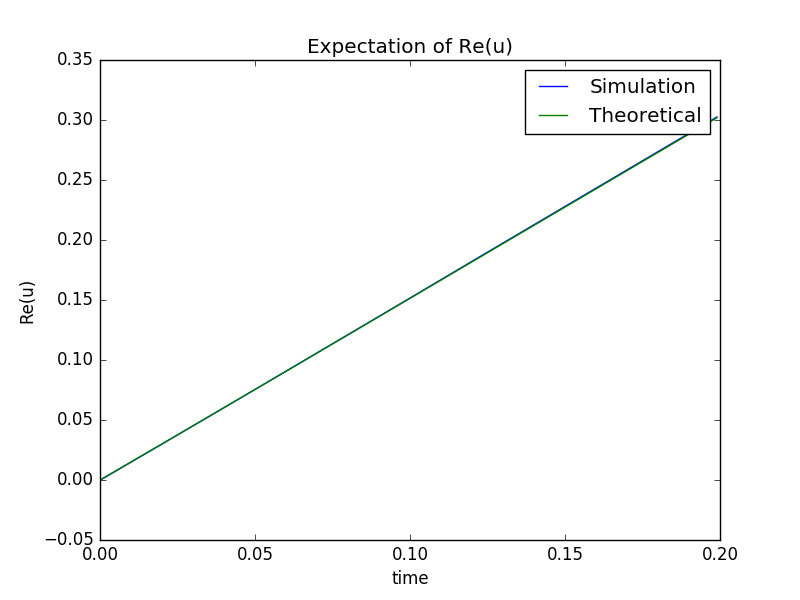
\includegraphics[width = 12cm]{NumericalSimulation/res/EuRe.png}
% \caption{Simulation of E[Re(u)]}
% \label{Simulation of E[Re(u)]}
% \end{figure}

% \begin{figure}[!ht]
% \centering
% 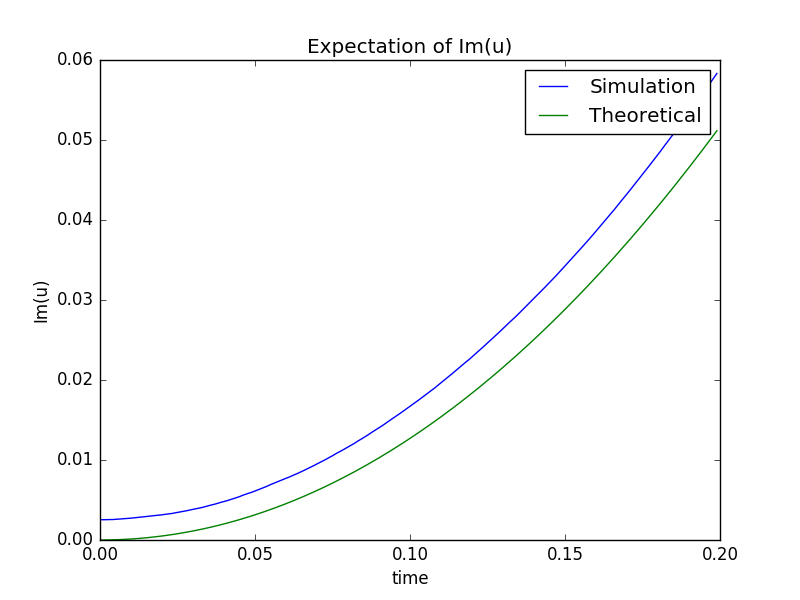
\includegraphics[width = 12cm]{NumericalSimulation/res/EuIm.png}
% \caption{Simulation of E[Im(u)]}
% \label{Simulation of E[Im(u)]}
% \end{figure}

% \begin{figure}[!ht]
% \centering
% 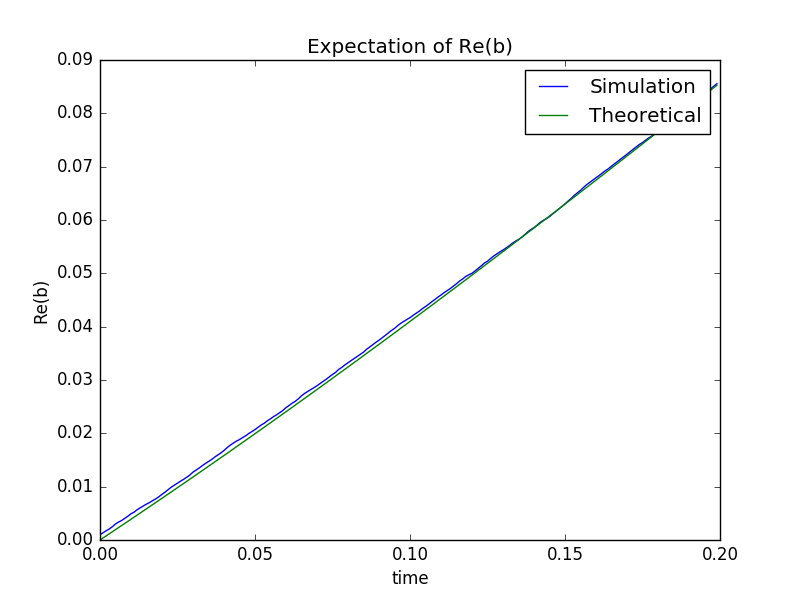
\includegraphics[width = 12cm]{NumericalSimulation/res/EbRe.png}
% \caption{Simulation of E[Re(b)]}
% \label{Simulation of E[Re(b)]}
% \end{figure}

% \begin{figure}[!ht]
% \centering
% 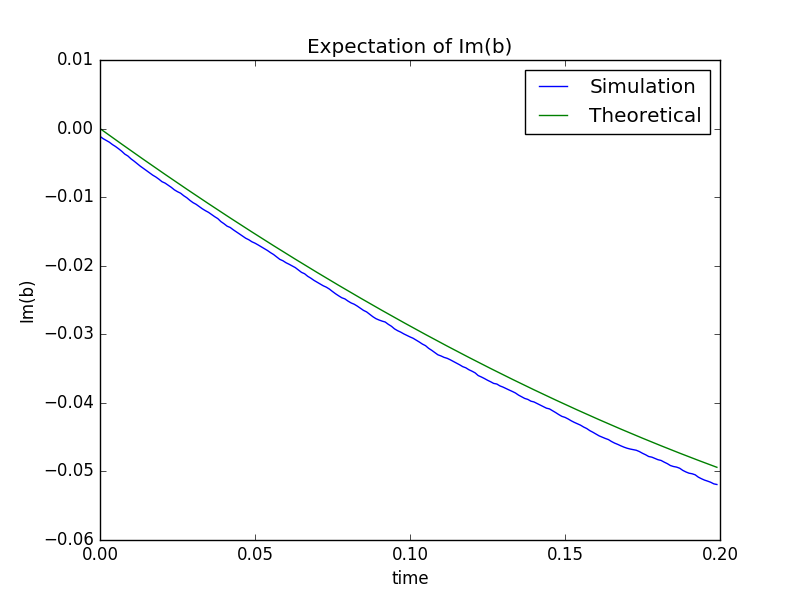
\includegraphics[width = 12cm]{NumericalSimulation/res/EbIm.png}
% \caption{Simulation of E[Im(b)]}
% \label{Simulation of E[Im(b)]}
% \end{figure}

% \begin{figure}[!ht]
% \centering
% 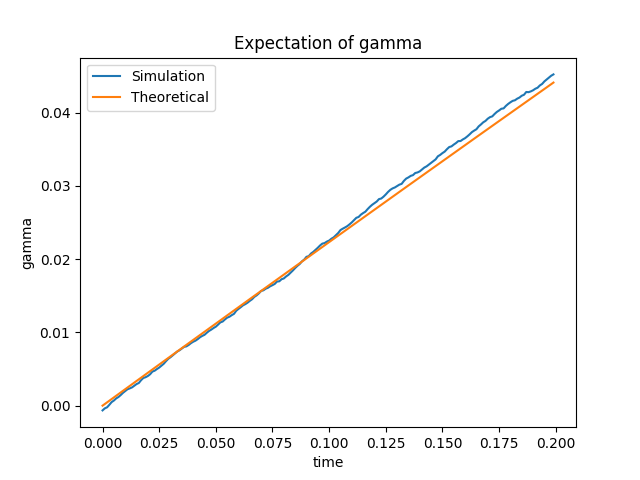
\includegraphics[width = 12cm]{NumericalSimulation/res/Egamma.png}
% \caption{Simulation of E[$\gamma$]}
% \label{Simulation of E[gamma]}
% \end{figure}

% \begin{figure}[!ht]
% \centering
% 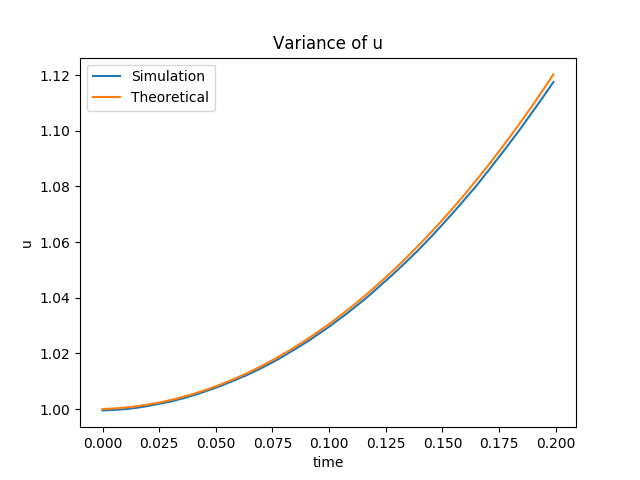
\includegraphics[width = 12cm]{NumericalSimulation/res/Varu.png}
% \caption{Simulation of Var(u)}
% \label{Simulation of Var(u)}
% \end{figure}

% \begin{figure}[!ht]
% \centering
% 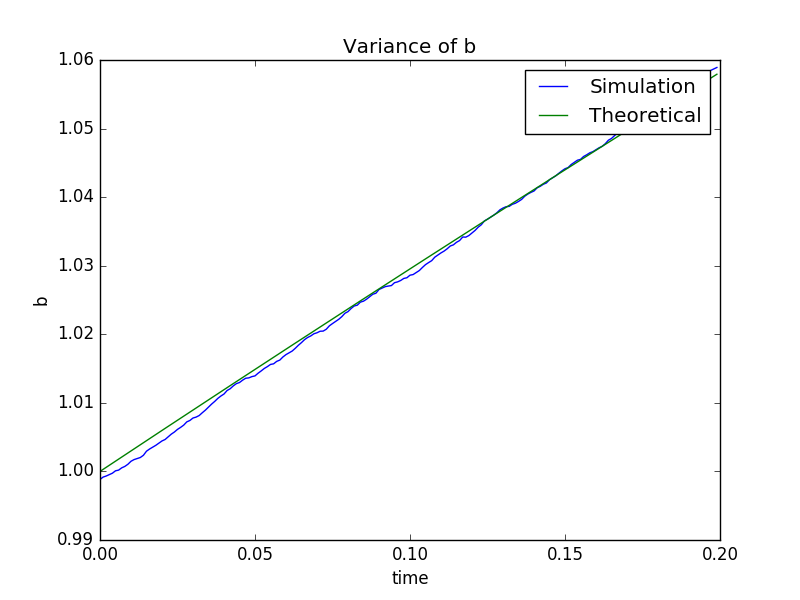
\includegraphics[width = 12cm]{NumericalSimulation/res/Varb.png}
% \caption{Simulation of Var(b)}
% \label{Simulation of Var(b)}
% \end{figure}

% \begin{figure}[!ht]
% \centering
% 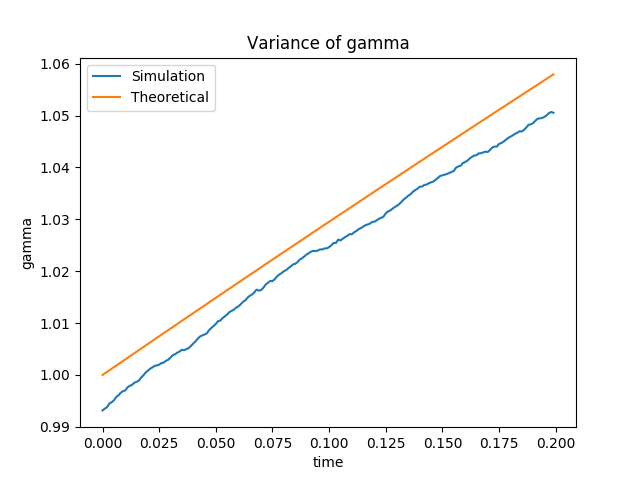
\includegraphics[width = 12cm]{NumericalSimulation/res/Vargamma.png}
% \caption{Simulation of Var($\gamma$)}
% \label{Simulation of Var(gamma)}
% \end{figure}

\begin{figure}[!ht]
\centering
\subfloat[\text{E}(Re(u))]{
  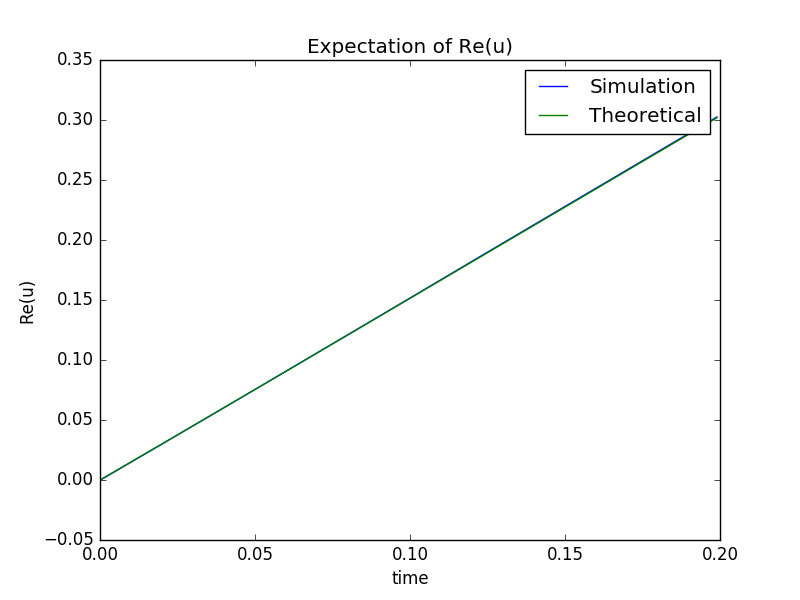
\includegraphics[width = .2\textwidth]{NumericalSimulation/res/EuRe.png}
  }\hfill
\subfloat[E(Im(u))]{
  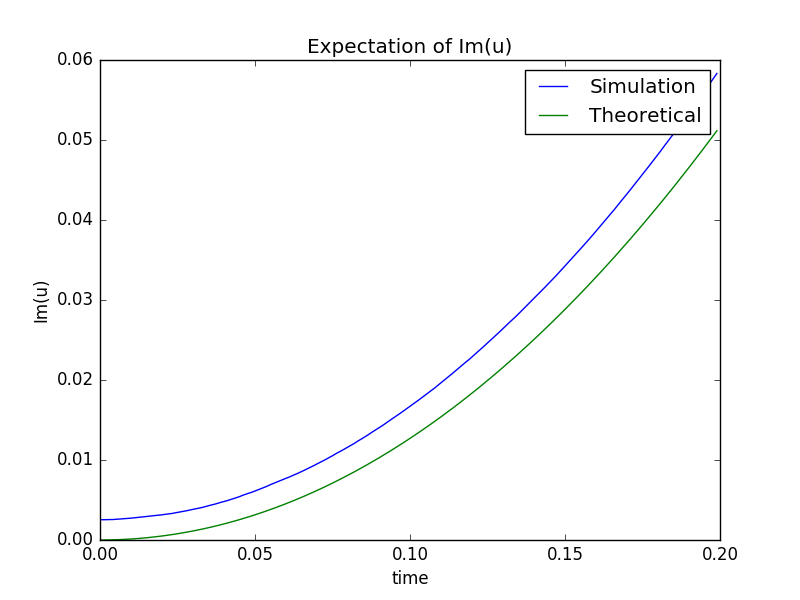
\includegraphics[width = .2\textwidth]{NumericalSimulation/res/EuIm.png}
  }\hfill
\subfloat[E(Re(b))]{
  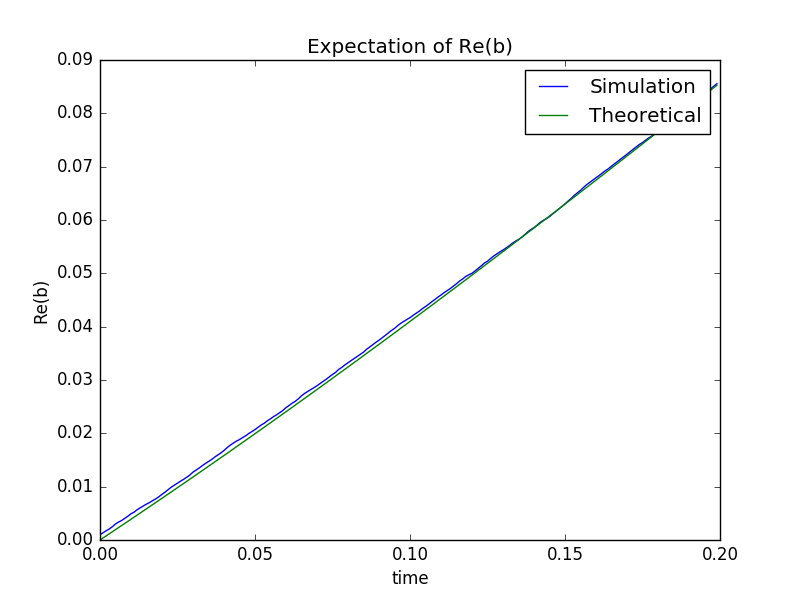
\includegraphics[width = .2\textwidth]{NumericalSimulation/res/EbRe.png}
  }\hfill
\subfloat[E(Im(b))]{
  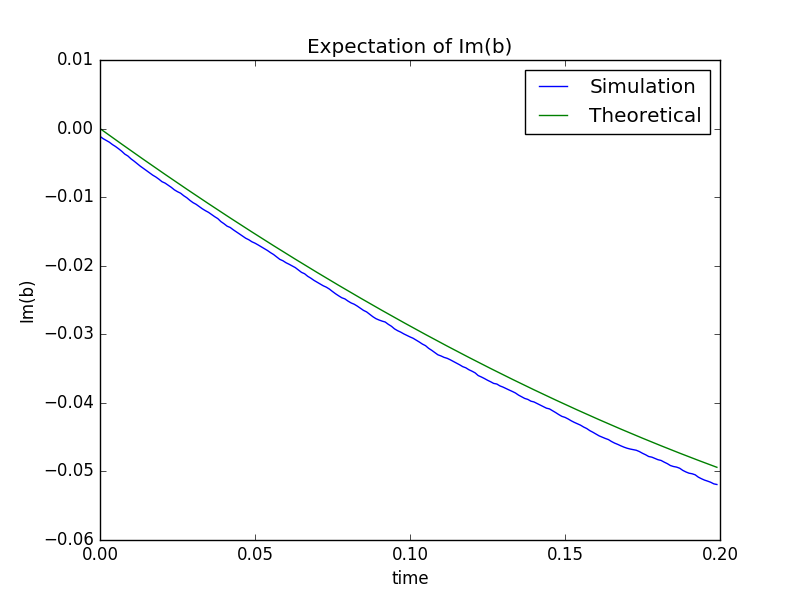
\includegraphics[width = .2\textwidth]{NumericalSimulation/res/EbIm.png}
  }\\
\subfloat[E($\gamma$)]{
  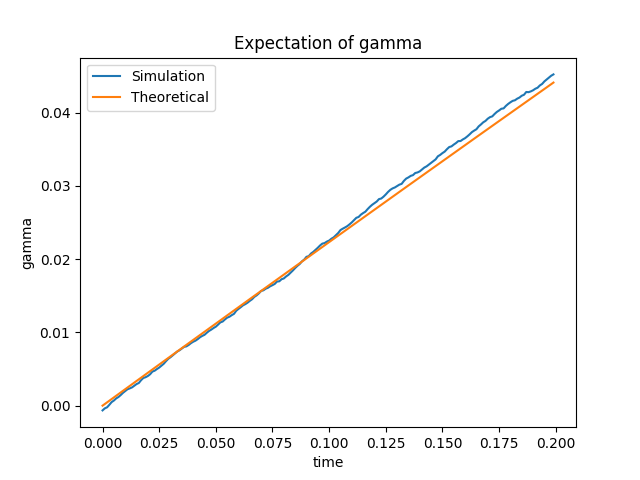
\includegraphics[width = .2\textwidth]{NumericalSimulation/res/Egamma.png}
  }\hfill
\subfloat[Var(u)]{
  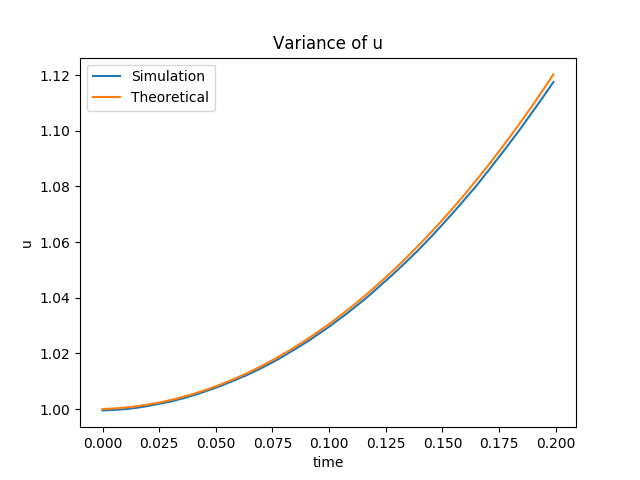
\includegraphics[width = .2\textwidth]{NumericalSimulation/res/Varu.png}
  }\hfill
\subfloat[Var(b)]{
  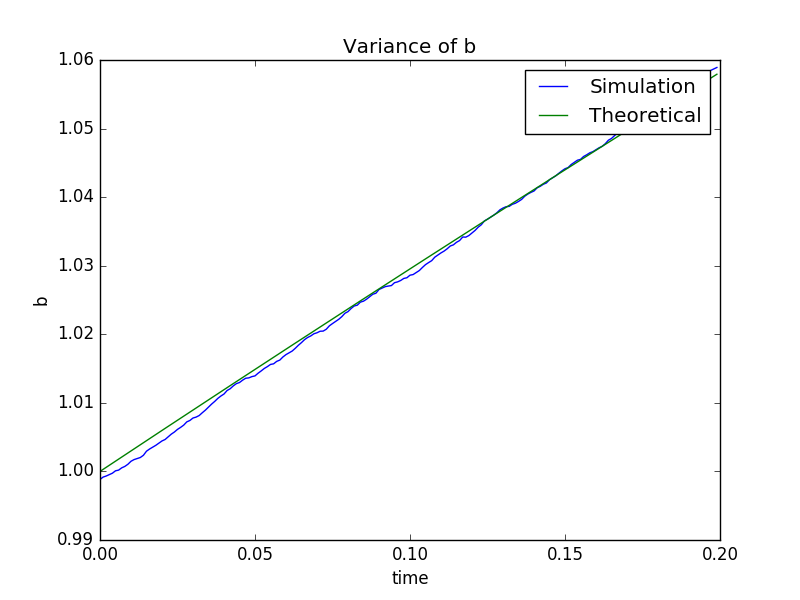
\includegraphics[width = .2\textwidth]{NumericalSimulation/res/Varb.png}
  }\hfill
\subfloat[Var($\gamma$)]{
  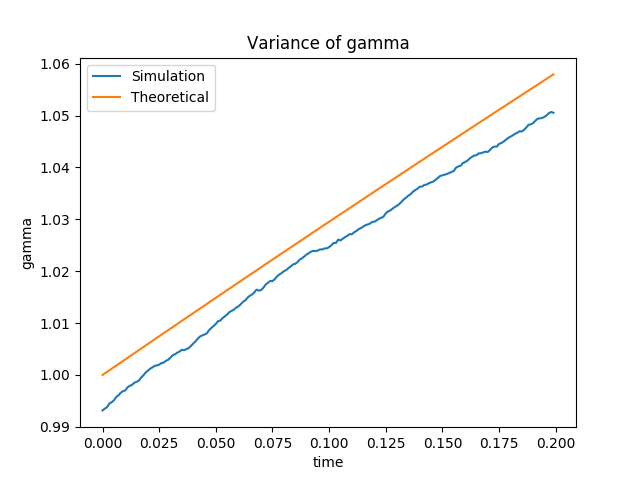
\includegraphics[width = .2\textwidth]{NumericalSimulation/res/Vargamma.png}
  }
\caption{Simulation of Expectations and Variances}
\label{Simulation of Expectations and Variances}
\end{figure}
\begin{figure}[!ht]
\centering
\subfloat[$\text{Re}(\Cov(u, u^*))$]{
  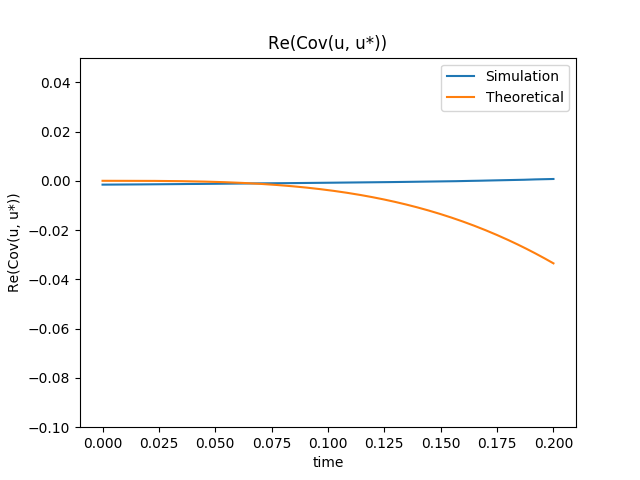
\includegraphics[width = .2\textwidth]{NumericalSimulation/res/lim/covuustarre.png}
}\hfill
\subfloat[$\text{Im}(\Cov(u, u^*))$]{
  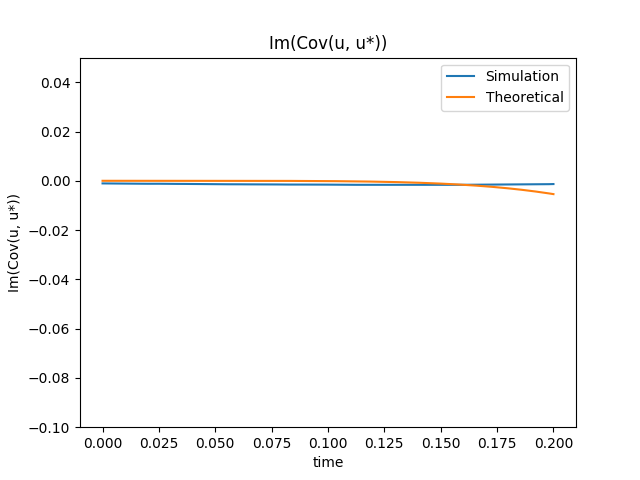
\includegraphics[width = .2\textwidth]{NumericalSimulation/res/lim/covuustarim.png}
}\hfill
\subfloat[$\text{Re}(\Cov(u, \gamma))$]{
  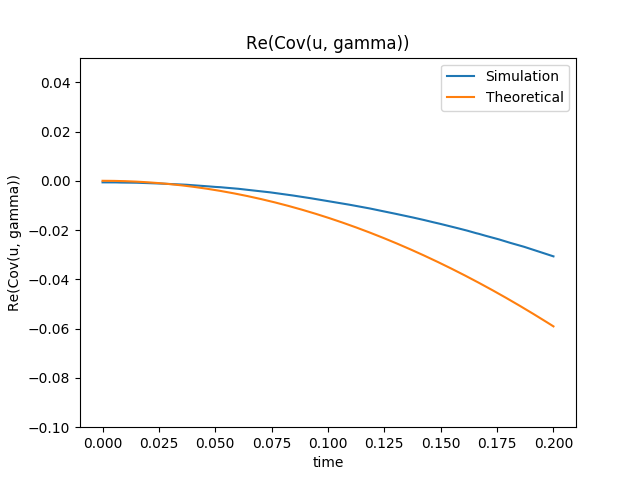
\includegraphics[width = .2\textwidth]{NumericalSimulation/res/lim/covugammare.png}
}\hfill
\subfloat[$\text{Im}(\Cov(u, \gamma))$]{
  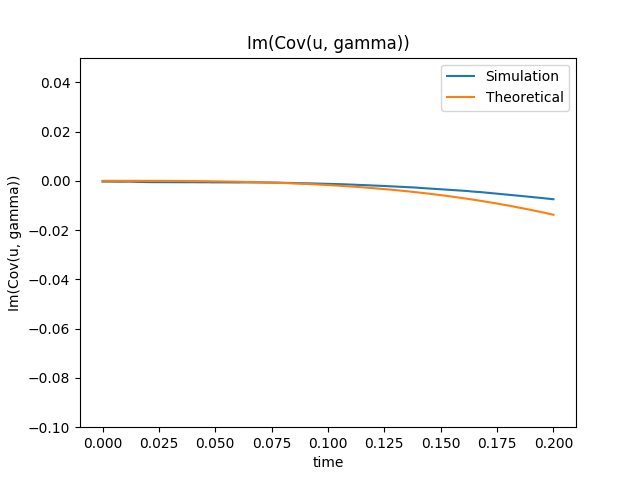
\includegraphics[width = .2\textwidth]{NumericalSimulation/res/lim/covugammaim.png}
}\\
\subfloat[$\text{Re}(\Cov(u, b))$]{
  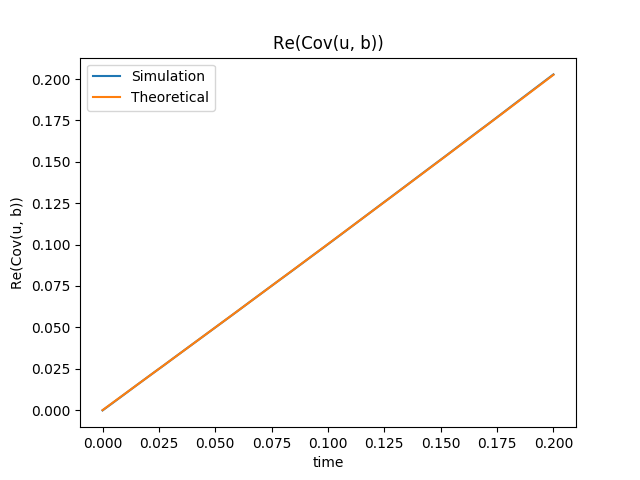
\includegraphics[width = .2\textwidth]{NumericalSimulation/res/lim/covubre.png}
}\hfill
\subfloat[$\text{Im}(\Cov(u, b))$]{
  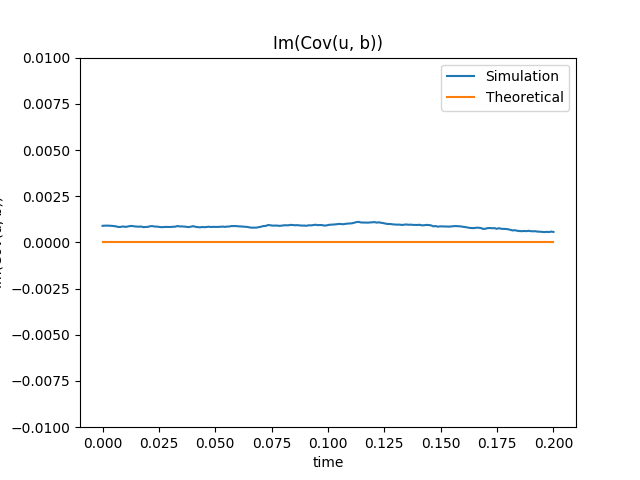
\includegraphics[width = .2\textwidth]{NumericalSimulation/res/lim/covubim.png}
}\hfill
\subfloat[$\text{Re}(\Cov(u, b^*))$]{
  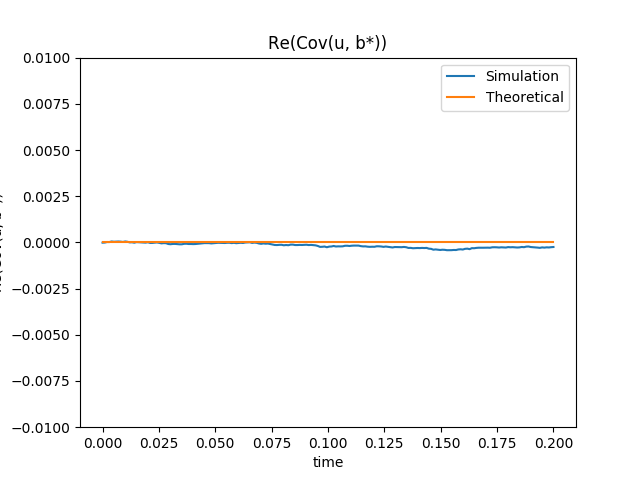
\includegraphics[width = .2\textwidth]{NumericalSimulation/res/lim/covubstarre.png}
}\hfill
\subfloat[$\text{Im}(\Cov(u, b^*))$]{
  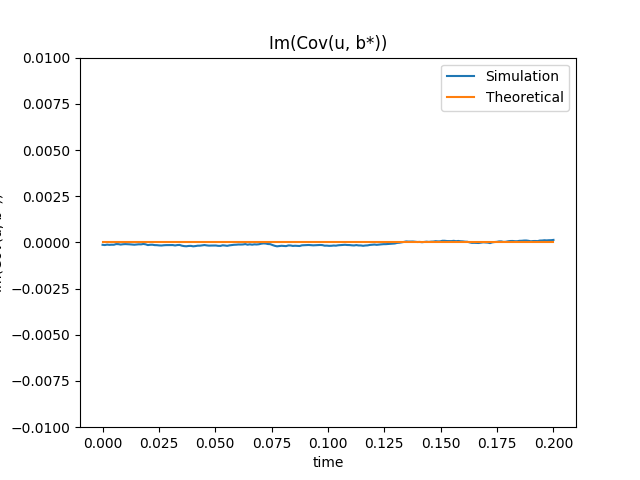
\includegraphics[width = .2\textwidth]{NumericalSimulation/res/lim/covubstarim.png}
}
\caption{Simulation of Covariances}
\label{Simulation of Covariances}
\end{figure}

\newpage


\subsection{讨论和展望}
在模拟结果中我们可以看到, 对期望和方差的模拟结果和理论结果均十分符合. 其中$\Var(b)$和$\Var(\gamma)$的模拟结果为一条和理论结果平行的曲线, 仅在初始时有截距上的误差, 这是由于初始值为随机变量所引起的. 

在协方差的模拟结果中我们可以发现, 如果我们将得到的图进行放大, 如下图所示:

\begin{figure}[!ht]
\centering
\subfloat[$\text{Re}(\Cov(u, u^*))$]{
  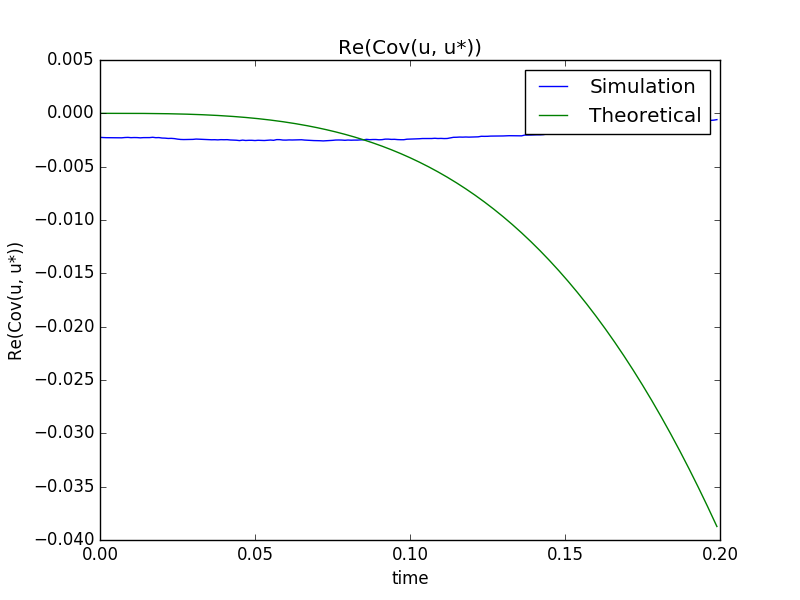
\includegraphics[width = .2\textwidth]{NumericalSimulation/res/CovuustarRe.png}
}\hfill
\subfloat[$\text{Im}(\Cov(u, u^*))$]{
  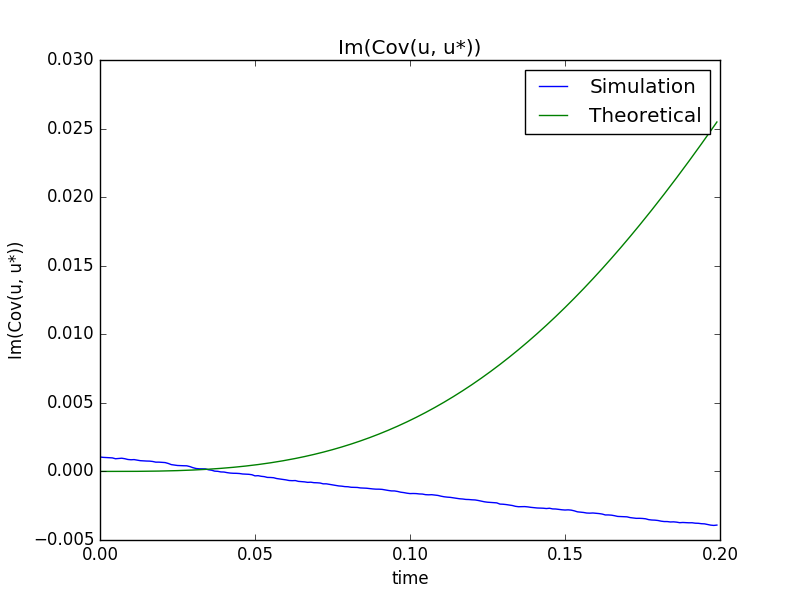
\includegraphics[width = .2\textwidth]{NumericalSimulation/res/CovuustarIm.png}
}\hfill
\subfloat[$\text{Re}(\Cov(u, \gamma))$]{
  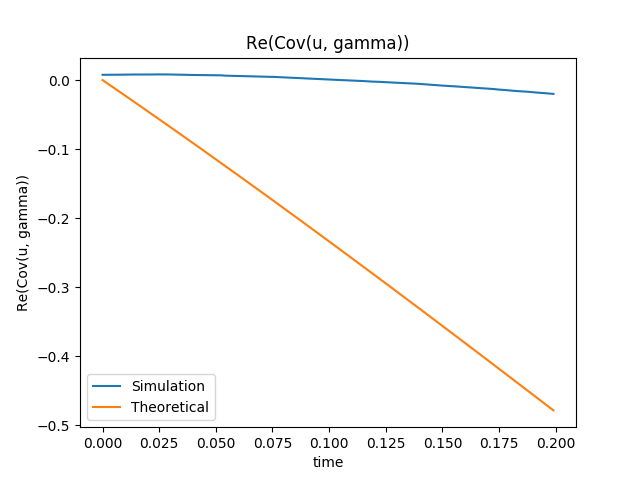
\includegraphics[width = .2\textwidth]{NumericalSimulation/res/CovugammaRe.png}
}\hfill
\subfloat[$\text{Im}(\Cov(u, \gamma))$]{
  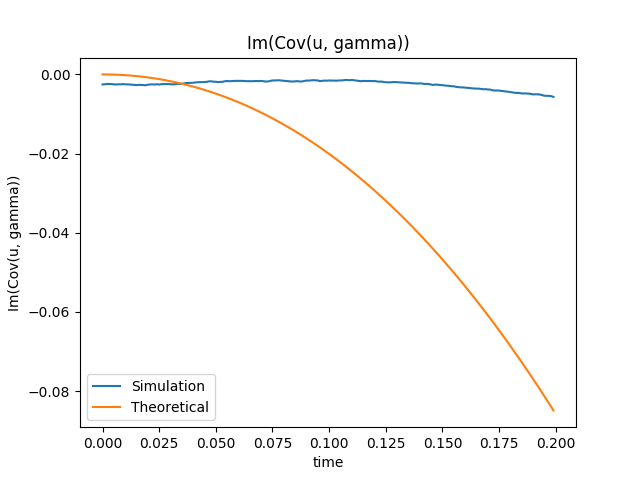
\includegraphics[width = .2\textwidth]{NumericalSimulation/res/CovugammaIm.png}
}\\
\subfloat[$\text{Re}(\Cov(u, b))$]{
  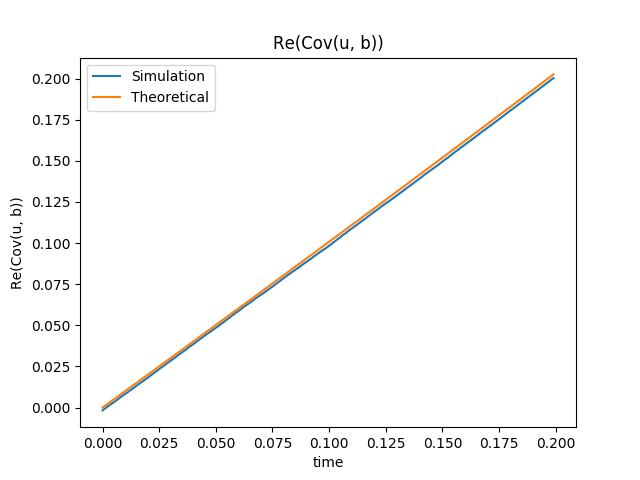
\includegraphics[width = .2\textwidth]{NumericalSimulation/res/CovubRe.png}
}\hfill
\subfloat[$\text{Im}(\Cov(u, b))$]{
  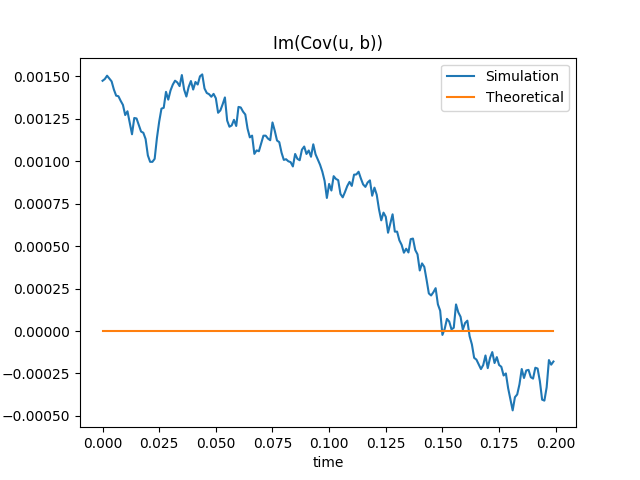
\includegraphics[width = .2\textwidth]{NumericalSimulation/res/CovubIm.png}
}\hfill
\subfloat[$\text{Re}(\Cov(u, b^*))$]{
  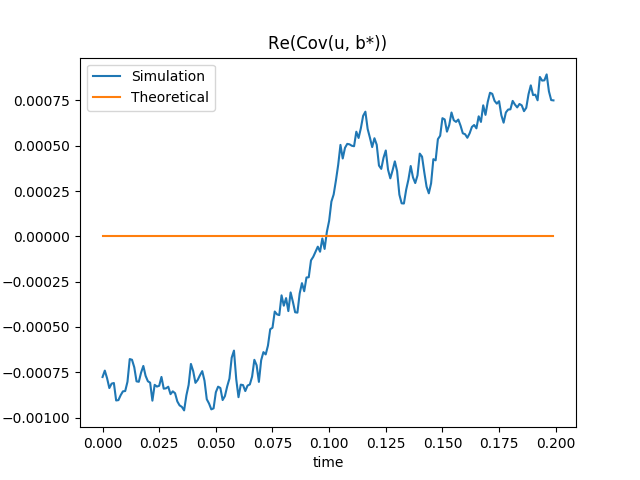
\includegraphics[width = .2\textwidth]{NumericalSimulation/res/CovubstarRe.png}
}\hfill
\subfloat[$\text{Im}(\Cov(u, b^*))$]{
  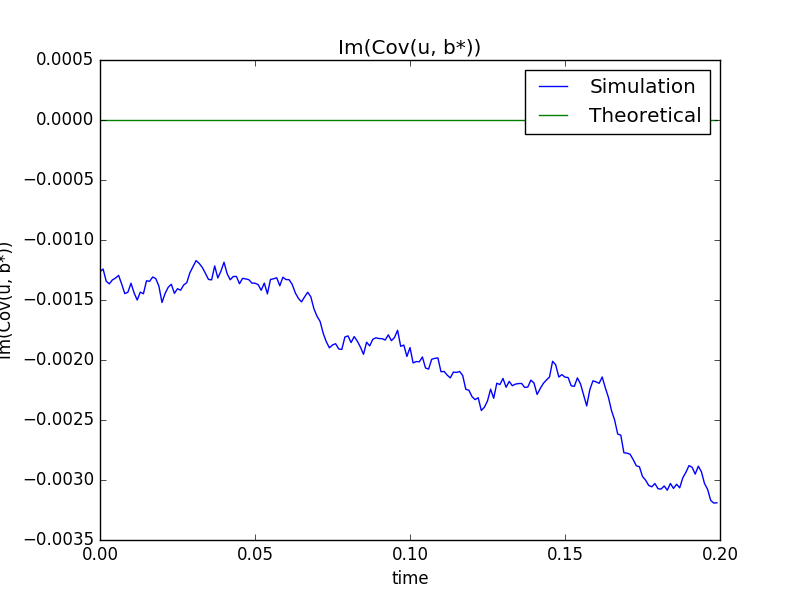
\includegraphics[width = .2\textwidth]{NumericalSimulation/res/CovubstarIm.png}
}
\caption{Simulation of Covariances, Detailed}
\label{Simulation of Covariances}
\end{figure}

我们可以发现, 对$\Cov(u, b)$和$\Cov(u, b^*)$的模拟结果在模拟100,000次时有$O(10^{-4})$的误差, 而对$\Cov(u, u^*)$和$\Cov(u, \gamma)$的模拟误差达到了$O(10^{-2})$的数量级. 根据分析\cite{golub2012matrix}, 这是因为复数运算时的条件数为实数运算的二次方, 故误差值也随之提高了两个数量级.

事实上, 根据相同的方法, 我们可以求出此随机微分方程组解的三节甚至四阶的统计量, 它们可以用初值和初始统计量的多重积分表示出来. 不过由于时间关系, 在这篇论文中没有将其详细的写出, 也没有对其进行数值上的模拟. 这些部分我们留待未来的研究中完成.
% \begin{figure}[!ht]
% \centering
% 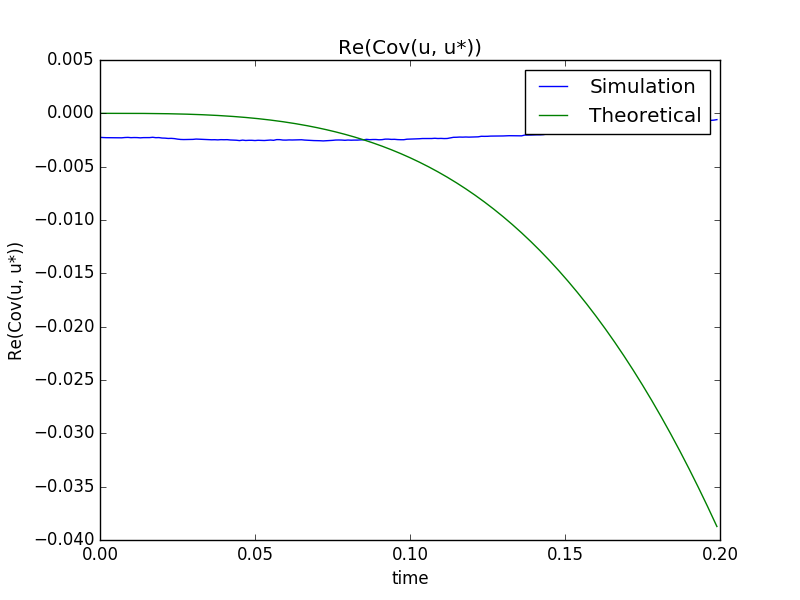
\includegraphics[width = 12cm]{NumericalSimulation/res/CovuustarRe.png}
% \caption{Simulation of $Re(Cov(u, u^*))$}
% \label{Simulation of Re(Cov(u, u*))}
% \end{figure}

% \begin{figure}[!ht]
% \centering
% 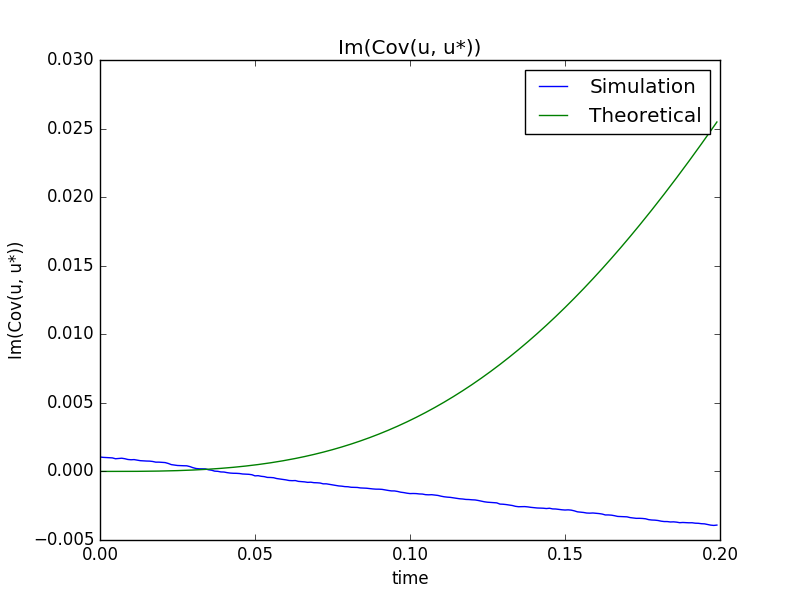
\includegraphics[width = 12cm]{NumericalSimulation/res/CovuustarIm.png}
% \caption{Simulation of $Im(Cov(u, u^*))$}
% \label{Simulation of Im(Cov(u, u*))}
% \end{figure}

% \begin{figure}[!ht]
% \centering
% 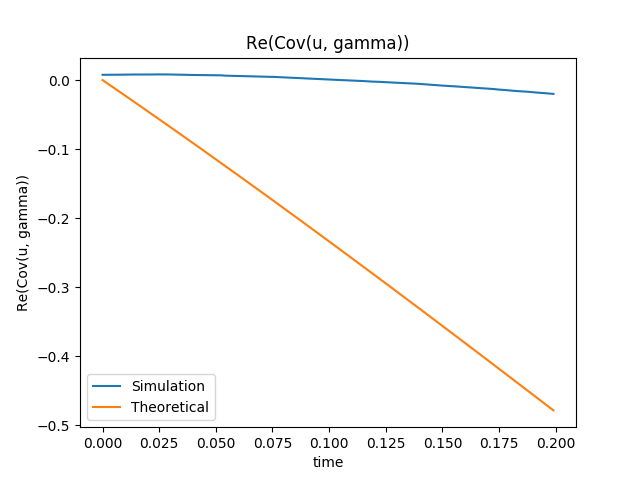
\includegraphics[width = 12cm]{NumericalSimulation/res/CovugammaRe.png}
% \caption{Simulation of $Re(Cov(u, \gamma))$}
% \label{Simulation of Re(Cov(u, gamma))}
% \end{figure}

% \begin{figure}[!ht]
% \centering
% 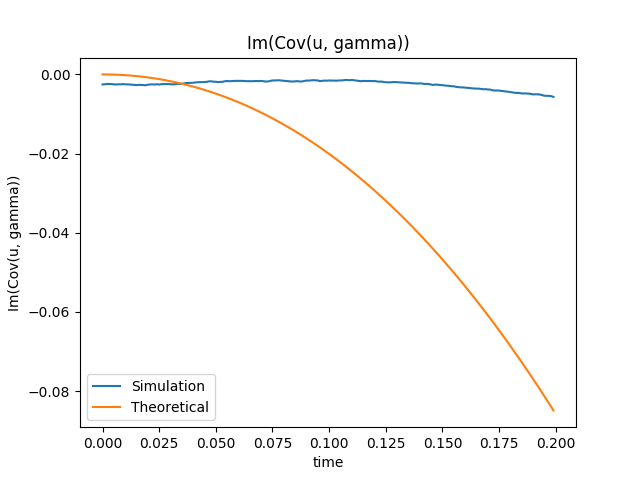
\includegraphics[width = 12cm]{NumericalSimulation/res/CovugammaIm.png}
% \caption{Simulation of $Im(Cov(u, \gamma))$}
% \label{Simulation of Im(Cov(u, gamma))}
% \end{figure}

% \begin{figure}[!ht]
% \centering
% 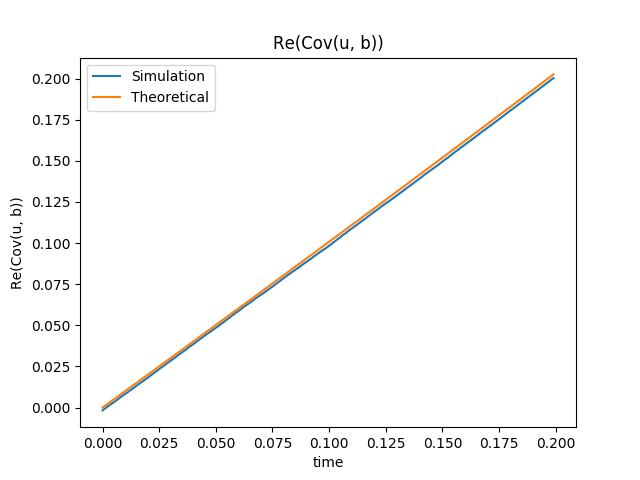
\includegraphics[width = 12cm]{NumericalSimulation/res/CovubRe.png}
% \caption{Simulation of $Re(Cov(u, b)$}
% \label{Simulation of Re(Cov(u, b)}
% \end{figure}

% \begin{figure}[!ht]
% \centering
% 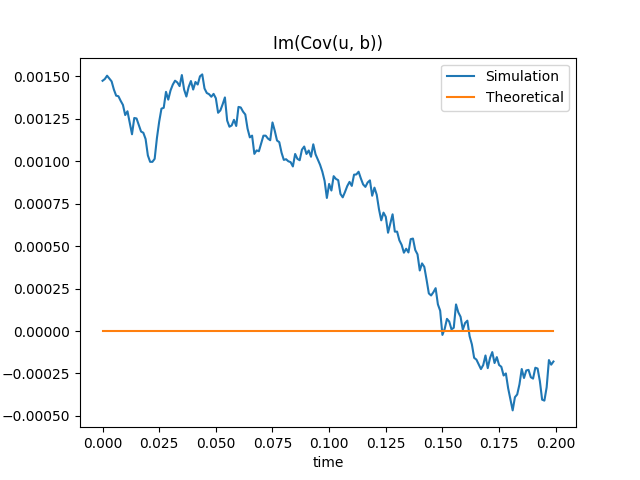
\includegraphics[width = 12cm]{NumericalSimulation/res/CovubIm.png}
% \caption{Simulation of $Im(Cov(u, b))$}
% \label{Simulation of Im(Cov(u, b))}
% \end{figure}

% \begin{figure}[!ht]
% \centering
% 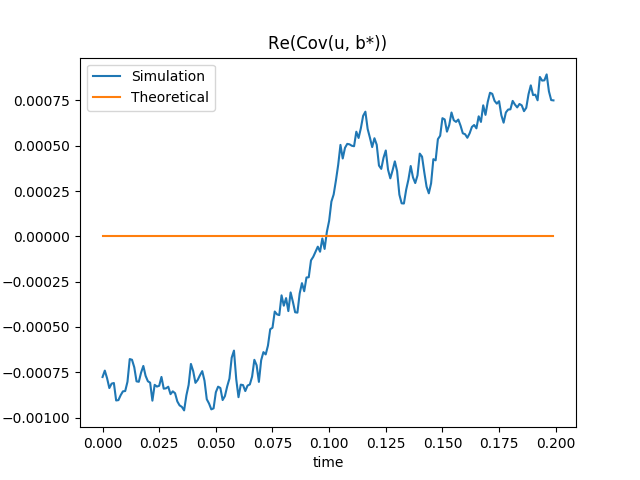
\includegraphics[width = 12cm]{NumericalSimulation/res/CovubstarRe.png}
% \caption{Simulation of $Re(Cov(u, b^*))$}
% \label{Simulation of Re(Cov(u, b*))}
% \end{figure}

% \begin{figure}[!ht]
% \centering
% 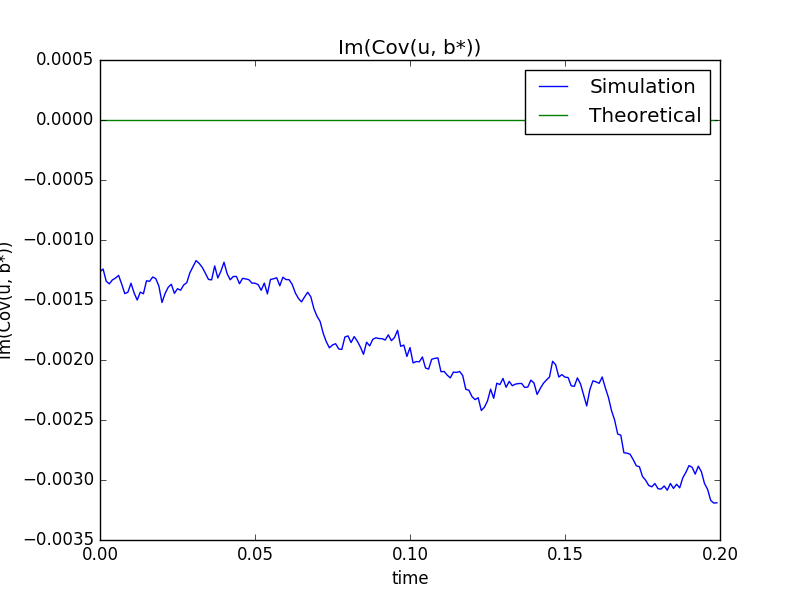
\includegraphics[width = 12cm]{NumericalSimulation/res/CovubstarIm.png}
% \caption{Simulation of $Im(Cov(u, b^*))$}
% \label{Simulation of Im(Cov(u, b*))}
% \end{figure}
\bibliographystyle{plain}
\bibliography{../../CONFIG/LaTeX-bib/Chuan}

\chapter*{\heiti 致谢}
\begin{flushleft}
感谢陆帅老师对本文研究方向的指导和帮助; \\
感谢宋杰承和唐博浩同学对本文理论和数值模拟的技术性建议; \\
感谢魏益民和赵冬华老师这一年来对我学习和研究的关心与支持; \\
感谢628的室友们, 数院和其他学院的同学们, 朋友和家人的陪伴; \\
最后, 感谢东区18和19号楼下的猫在最困难的的日子里给予我的慰藉.
\end{flushleft}
\end{document}{}